\documentclass[169, handout	]{THIbeamer} % for print add handout
\usepackage{biblatex}

\usepackage[utf8]{inputenc}
\usepackage[greek,ngerman]{babel}
\usepackage{hyperref}
\usepackage{multimedia}
\usepackage{csquotes}

% Table
\usepackage{hhline}
\usepackage{multirow}

% Figures
\usepackage{subcaption}
\captionsetup[subfigure]{justification=justified,singlelinecheck=false}
\graphicspath{{Images/}}

% Math
\usefonttheme[onlymath]{serif}
\usepackage{amsmath}
\usepackage{units}


% Tikz
\usepackage{tikz}
\usetikzlibrary{backgrounds,shadows,arrows}%external
\usepackage{pgfplots}
\usepackage{pgfgantt}
\usepackage{pdflscape}
\pgfplotsset{compat=newest}
%Only compile figures when something has changed
%\tikzexternalize[prefix=TikzPictures/]
\title{Summercamp 2022}

\newcommand{\argmin}{\mathop{\mathrm{arg\,min}}}
\subtitle{Projekt Automatisiertes Fahren}

\date{01.03.2022}

\author{Karthikeyan Chandra Sekaran}


\begin{document}
	\begin{frame}[plain]
		\maketitle
	\end{frame}
	\begin{frame}{Outline}
		\begin{minipage}{0.4\textwidth}
			\begin{enumerate}
				\item Szenariobeschreibung
				\item Sensor Setup
				\begin{enumerate}
					\item LiDAR
					\item ADMA
				\end{enumerate}
				\item Datenverarbeitung
				\begin{enumerate}
					\item ROS
					\item Region of Interest
					\item Ground Subtraction
					\item Clustering		
				\end{enumerate}
			\item[]
			\end{enumerate}
		\end{minipage}%
		\hfill
		\begin{minipage}{0.5\textwidth}
		\begin{tabular}{p{\textwidth}}
			\begin{enumerate}
				\setcounter{enumi}{4}	
				\item KI-Algorithmus 				
				\begin{enumerate}
					\item Grundlagen des Maschinellen Lernens
					\item Ermittlung der kritischen Zeit	
					\item Lineare Regression 
					\item Nicht-lineare Basisfunktionen 
				\end{enumerate}	
				\item Verwendung der Algorithmen in einer Echtzeit-Anwendung
			\end{enumerate}
		\end{tabular}
		\end{minipage}%
	\end{frame}
	\begin{frame}{Szenariobeschreibung}
		Das mit LiDAR- und ADMA-Sensorik ausgestattete Ego-Fahrzeug folgt einem Fahrzeug der gleichen Spur, welches überraschend eine Notbremsung einleitet. Um den Auffahrunfall zu verhindern, ist der kritsche Zeitpunkt $t_{\text{crit}}$ zu bestimmen, zu dem das Ego-Fahrzeug spätestens seine Bremsung einleiten muss.
		\\
		\textbf{Ziele:} \\
		\begin{enumerate}
			\item Verarbeitung der Sensorrohdaten des Szenarios
			\item Entwicklung eines KI-Algorithmus zur Ermittlung der kritischen Zeit $t_{\text{crit}}$.
			\item Anwendung der Algorithmen in einer Echtzeit-Simulation des Szenarios.
		\end{enumerate}
	\end{frame}
	\begin{frame}{Fragen zur Szenariobeschreibung}
		\begin{figure}

			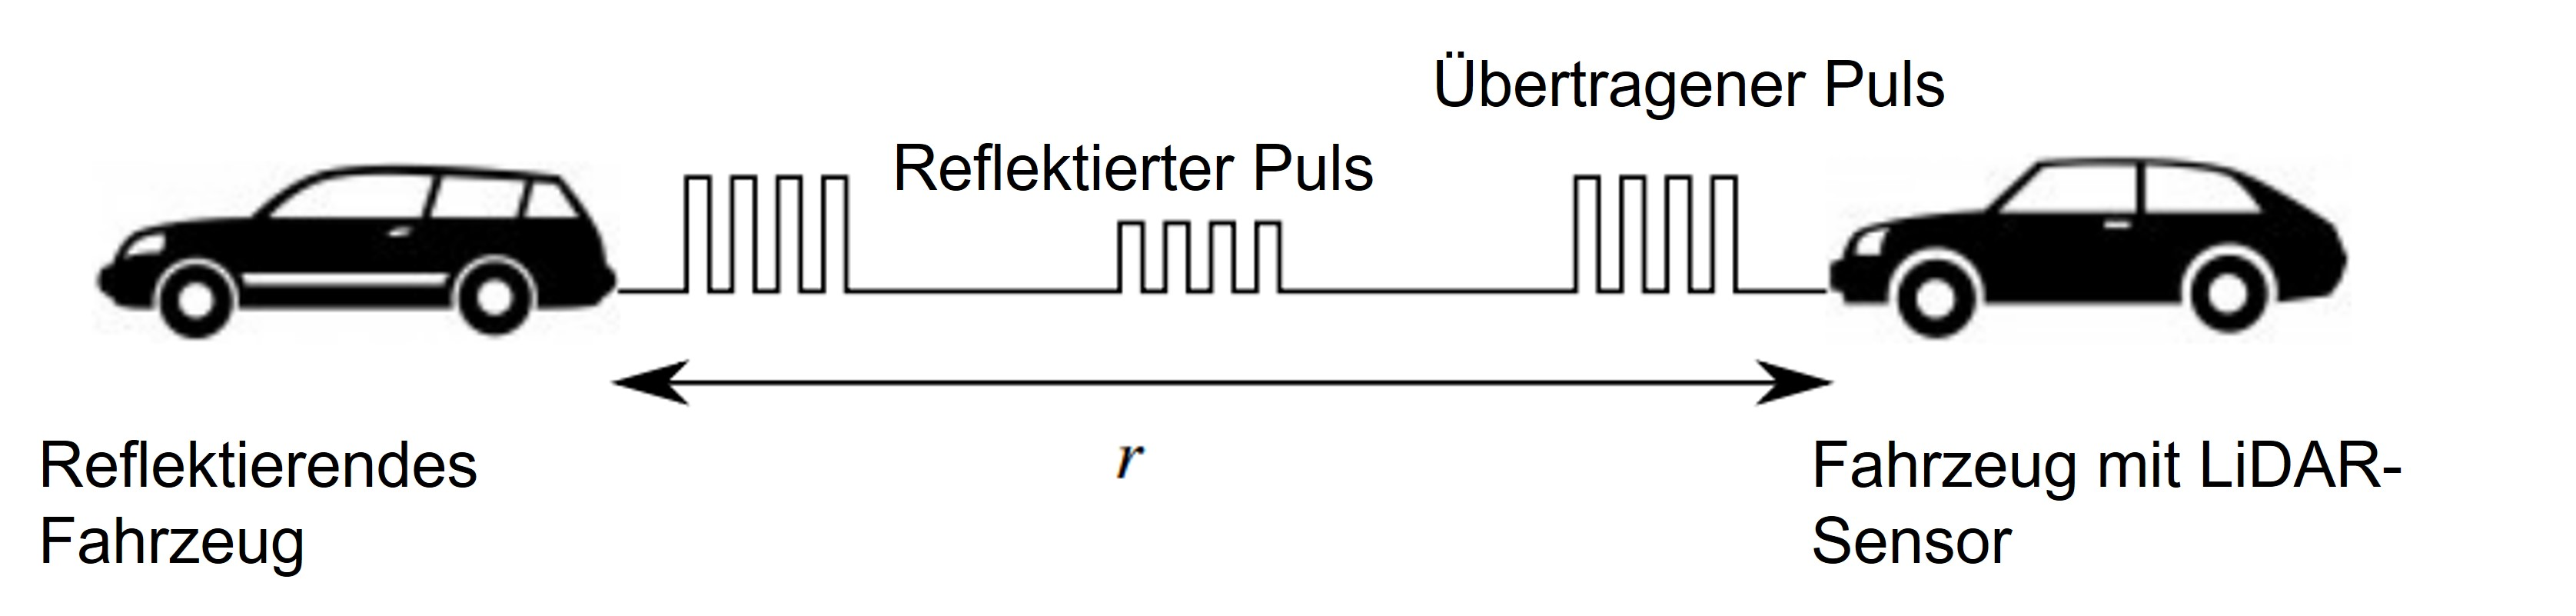
\includegraphics[scale=0.4]{"required/Szenariobeschreibung_auto.jpg"}

		\end{figure}	
		\textbf{Fragen:}\\
		\begin{enumerate}
			\item Welche Assistenzsysteme sind in Fahrzeugen mit LiDAR-Sensoren vorstellbar?
			\item Welches Assistenzsystem könnte mit diesem Aufbau erprobt werden?
			\item Wie kann die Implementierung eines Assistenzsystems aussehen? Welche Eingangsgrößen benötigt die Entscheidungslogik?
		\end{enumerate}
	\end{frame}
	\begin{frame}{Sensor Setup}{Lidar Sensor}
		\textbf{LiDAR}...		
		\begin{itemize}
			\item ... steht als Akronym für \enquote{Light Detection And Ranging}
			\item ... ist ein optisches Verfahren zur Messung von Distanzen
			\item ... sendet optisches Laserlicht in Pulsen aus. 
			\item ... arbeitet mit Wellenlängen nahe des sichtbaren Bereichs ($\mu m$-Wellen)
		\end{itemize}
		\textbf{Visualisierung} des Lidar-Prinzips [Wik.2022]
		\begin{figure}[htbp]
    		\centering
    		\begin{subfigure}[b]{0.15\textwidth}
        		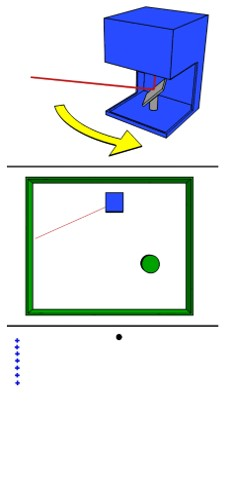
\includegraphics[scale=0.2]{required/LiDAR-Sensor1.jpg}
        		\label{Lidar-t1}
   		 	\end{subfigure}
    		\begin{subfigure}[b]{0.15\textwidth}
       		 	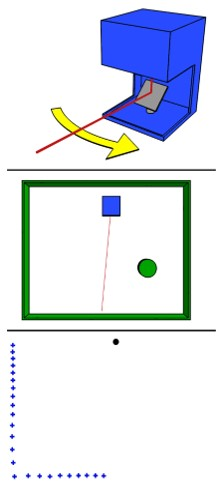
\includegraphics[scale=0.2]{required/LiDAR-Sensor2.jpg}
        		\label{Lidar-t2}
    		\end{subfigure}
   	 		\begin{subfigure}[b]{0.15\textwidth}
        		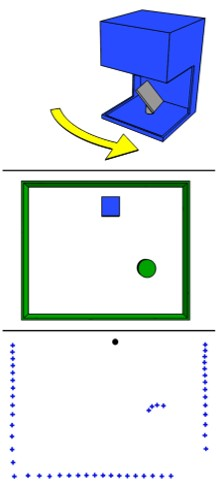
\includegraphics[scale=0.2]{required/LiDAR-Sensor3.jpg}
        		\label{Lidar-t3}
    		\end{subfigure}
    		\label{Lidar in Raum}
		\end{figure}
	\end{frame}
	
	\begin{frame}{Sensor Setup}{LiDAR Sensor}
		\begin{itemize}
			\item \textbf{Distanzmessung} per \enquote{time-of-flight}-Prinzip:
			\begin{itemize}
				\item Sende und Empfangszeit des Pulses wird gemessen
				\item Aus der Zeitdifferenz $\Delta t$ und der Geschwindigkeit des Lichts $ c = 3 \cdot 10^{8} \frac{m}{s} $
				\begin{equation}
					r = \frac{c}{2} \cdot \delta t
				\end{equation}
			\end{itemize}
			\item \textbf{Geschwindigkeitsbestimmung:} Nur indirekt auf Basis von Signalverarbeitungstechniken aus der Distanzmessung ableitbar
			\item \textbf{Vorteile}: Großer Öffnungswinkel, Detektion aller möglichen Objekte (ohne Training, da aktiver Sensor), Klassifizierung von Objekten möglich, etc.
			\item \textbf{Nachteile:} Wetteranfälligkeit, keine direkte Geschwindigkeitsmessung, etc.
		\end{itemize}
	\end{frame}
	\begin{frame}{Sensor Setup}{LiDAR Sensor: Rohdaten Ausgabe}
		\begin{itemize}
			\item \textbf{Ausgabeformat:} [$x, y, z, int, t$] $\rightarrow$ $N \times 4$ Matrix für eine Punktwolke mit $N$ Punkten
			\item \textbf{Speicheranforderungen} am Beispiel des Velodyne HDL-64E (rotierender 3D Laserscanner, der z.B. im  Open-Source Kitti-Datensatz verwendet wird):
			\begin{itemize}
				\item Sichtfeld: 360° horizontal, 36.8° vertikal | Reichweite: 120 m | Frequenz: 10 Hz
				\item Ausgegebene Punkte: $~ 1.3 \cdot 10^{6}$ $\frac{\text{pts}}{\text{s}}$ 
				\item Benötigter Speicher: $~1.8$ $\frac{\text{MB}}{\text{Frame}} \cdot 10$ $\frac{\text{Frames}}{\text{s}} = 18$  $\frac{\text{MB}}{\text{s}}$
			\end{itemize}			 
			\item \textbf{Beispiel:}
		\end{itemize}					
		\begin{figure}
			\includegraphics[scale=0.3]{required/LiDAR auf Parkplatz.jpg}
			\caption{LiDAR-Aufnahme auf einem Parkplatz [Rummelhard.2017]}
		\end{figure}
	\end{frame}
	\begin{frame}{Sensor Setup}{ADMA Sensor}
		\textbf{ADMA}...		
		\begin{itemize}
			\item ... steht als Akronym für \enquote{Automotive Dynamic Motion Analyzer}
			\item ... setzt sich aus IMU, GNSS und einem Prozessor zusammen und kann somit Geschwindigkeit, räumliche Lage des Fahrzeugs und Standort in Echtzeit ausgeben
		\end{itemize}
		\begin{figure}
			\centering
    		\begin{subfigure}[b]{0.3\textwidth}
				\includegraphics[scale=0.35]{required/ADMA-Erklärung.jpg}
				\caption{ADMA als \enquote{Sinnesorgan} des Fahrzeugs [AD14]}
        		\label{ADMA Erklärung}
   		 	\end{subfigure}
   		 	\hspace{3cm}
    		\begin{subfigure}[b]{0.3\textwidth}
				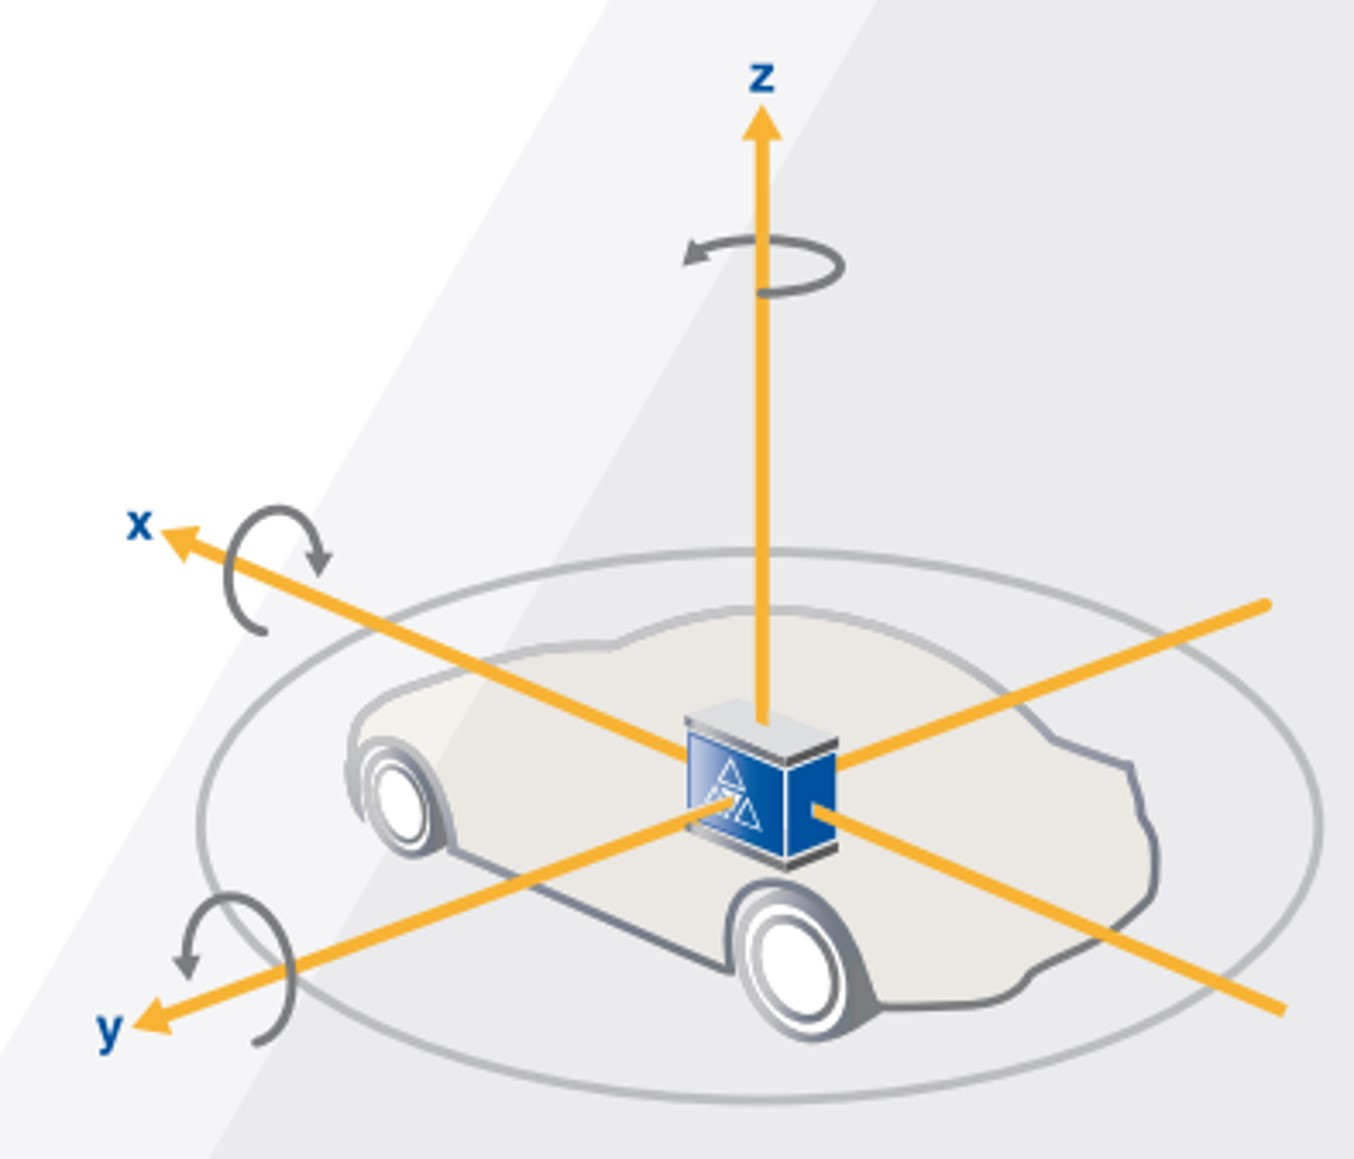
\includegraphics[scale=0.35]{required/ADMA.jpg}
				\caption{ADMA im Fahrzeug [GeneSys.2022]}
        		\label{ADMA in Fahrzeug}
    		\end{subfigure}
    		\label{ADMA figures} 
		\end{figure}
	\end{frame}
	\begin{frame}{Datenverarbeitung}{Erläuterung}
		\textbf{Motivation:} 
		\begin{itemize}
			\item Filtern von störenden oder für den Verwendungszweck nicht relevanten Anteile
			\item Reduktion des Speicher- und Rechenbedarfs in folgenden Algorithmen
			\item Ausgabe der Daten entsprechend der Schnittstellenanforderungen folgender Algorithmen
			\item Nutzen von A-Priori Wissen zur Verkleinerung des ausgewerteten Lösungsraums für folgende Alogrithmen $\rightarrow$ Algorithmus muss diese Eingrenzung nicht mehr erlernen
			\item Erfüllung der Echzeitanforderungen
		\end{itemize}
		\textbf{Aufgabenstellung:} Ausgabe der Punktewolke für die wichtigen Objekte der Aufnahme
	\end{frame}
	\begin{frame}{Datenverarbeitung}{Erläuterung}
		\textbf{Vorgehensweise:} 
		\begin{enumerate}
			\item \enquote{Region of Interest}-Filterung: Filterung der für den Verwendungszweck unrelvanten Daten
			\item \enquote{Ground Subtraction}: Filterung der Lidarpunkte der Fahrbahnfläche
			\item \enquote{Clustering}: Segmentierung zusammenhängender Punkte 
			\item \enquote{Objekterkennung}: Ausgabe von Objekten auf Basis der Clustergrenzen
		\end{enumerate}
		\vspace{0.5cm}
		Eine genauere Erläuterung zu den einzelnen Schritten wird in den folgenden Kapiteln gegeben.
	\end{frame}	
	\begin{frame}{Datenverarbeitung}{Erläuterung ROS}				
		\textbf{Motivation}: 
		\begin{itemize}
			\item bietet Struktur, Tools und Algorithmen für die Implementierung eigener Applikationen
			\item Sensorausgabe kann in dieses System eingebunden und somit verarbeitet werden
		\end{itemize}		
		\textbf{Allgemein}:
		\begin{itemize}
			\item Open-Source Framework
			\item Aufgaben: Hardwareabstraktion, Hilfsfunktionen, Interprozesskommunikation, Gerätetreiber, Paketmanagement
		\end{itemize}		
		\begin{figure}
			\centering
    		\begin{subfigure}[b]{0.4\textwidth}
				
\includegraphics[scale=0.3]{required/ROS.jpg}
				\caption{ROS: Noetic Ninjemys [ROS.2022]}
        		\label{ROS}
   		 	\end{subfigure}
    		\begin{subfigure}[b]{0.4\textwidth}
				
\includegraphics[scale=0.3]{required/ROS2.jpg}
				\caption{ROS 2: Humble Hawksbill [ROS.2022]}
        		\label{ROS}
    		\end{subfigure}
		\end{figure}			
	\end{frame}
	\begin{frame}{ROS}{Aufbau}
		\footnotesize
		\begin{itemize}
			\item \textbf{ROS Nodes}: Eigenständige Programme, die ihre vorgebene Logik ausführen
			\item \textbf{ROS Master}: Zentraler Haupt-Knoten im System $\rightarrow$ kennt die Nodes des Systems und ermöglicht dadurch die Kommunikation zwischen der LiDAR-Sensor Node und der Datenverarbeitungs-Node.
			\item \textbf{ROS Topic}: eigener \enquote{Kommunikationskanal}, wodurch die Erzeugung und Nutzung von Information entkoppelt ist
			\item \textbf{ROS Messages}: Definieren die Daten die ROS Nodes über Topics kommuinizieren
			\item Serviceorientierte Architektur, die mit Publisher-Subscriber Beziehungen arbeitet
			\item Programmiersprachen: C++, Python 
		\end{itemize}				
		\begin{figure}
			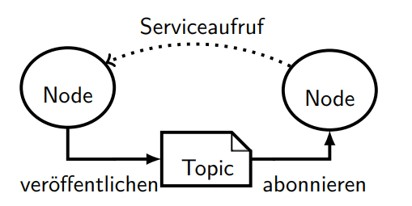
\includegraphics[scale=0.35]{required/ROS-Aufbau.jpg}
			\caption{Darstellung der Kommuikation zwischen Nodes in ROS}
		\end{figure}
	\end{frame}
	\begin{frame}{ROS}{Ordnerstruktur}
		\begin{figure}
			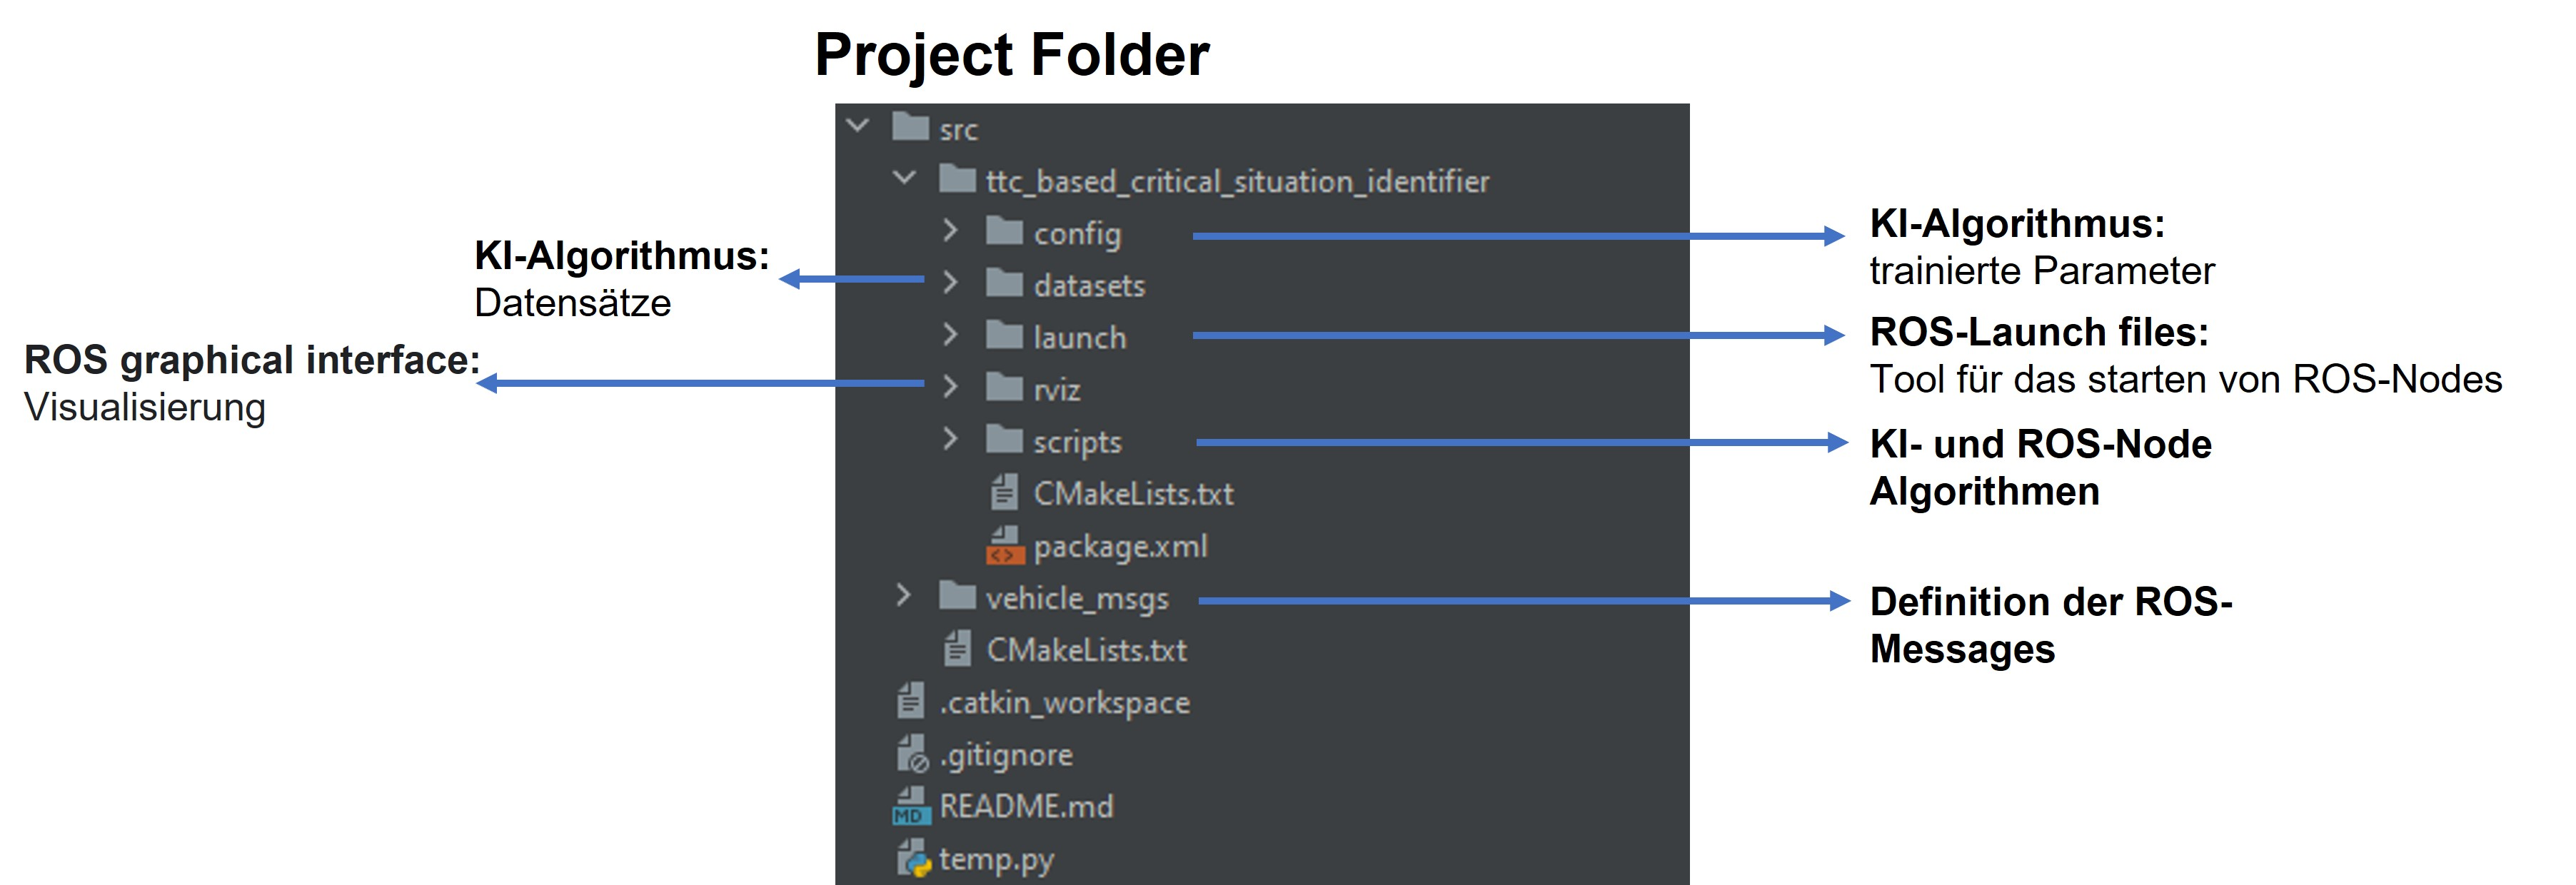
\includegraphics[scale=0.5]{required/ROS_Folder_Structure.jpg}
			\caption{Darstellung der Ordnerstruktur}
		\end{figure}
	\end{frame}
	\begin{frame}{Datenverarbeitung}{Erläuterung der geplanten Architektur}
		\begin{figure}
			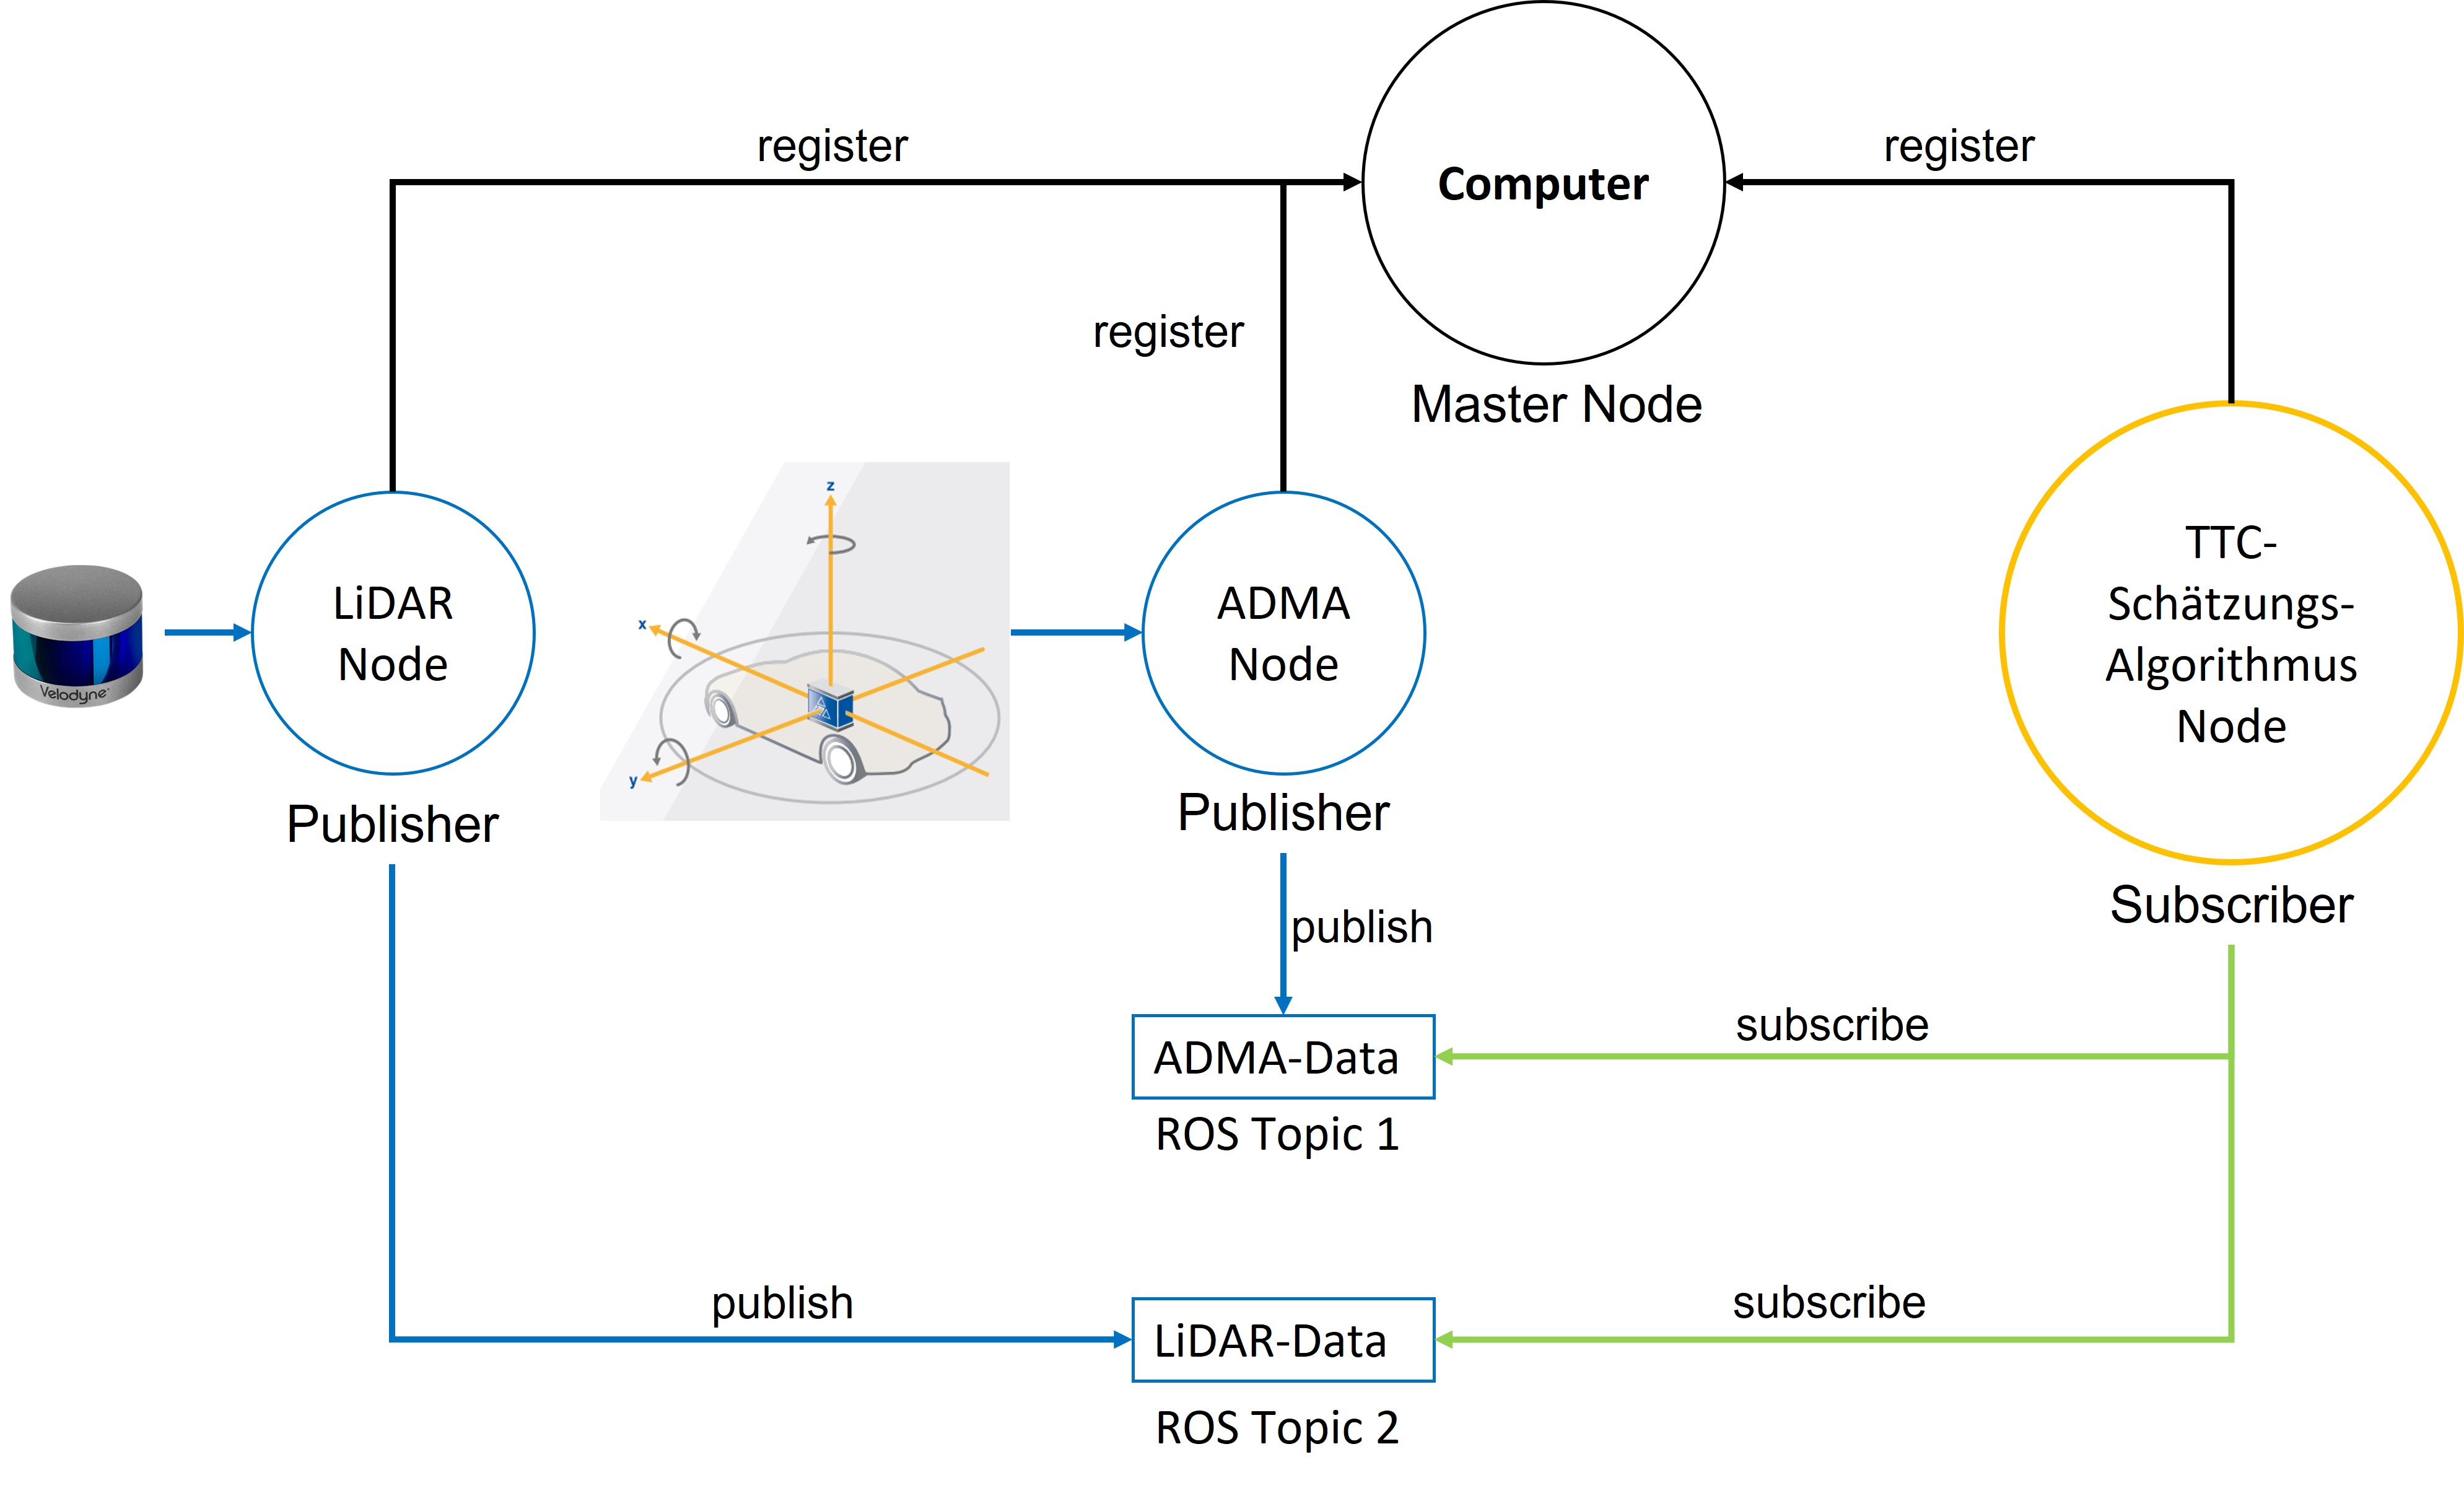
\includegraphics[scale=0.35]{required/ROS_Architecture.jpg}
			\caption{Darstellung der ROS Architektur des Szenarios}
		\end{figure}
	\end{frame}
	\begin{frame}{Datenverarbeitung}{Implementierung: Region of Interest}
		\textbf{Motivation}
		\begin{itemize}
			\item Je nach Algorithmus ist nur ein Teil des Datensatzes für dessen Auswertung relevant
			\item Beispiel für A-Piori Wissen im automatisierten Fahren: HD-Maps
			\begin{itemize}
				\item Im Fahrzeug verfügbare Information über die Umgebung
				\item Daraus ableitbar: Regionen mit möglichem Verkehrsaufkommen und potentielle Gefahrenbereiche
				\item Folgerung: gezielte Reduktion des ausgewerteten Datenraums auf den für den Algorithmus relevanten Bereich
				\item Beispiel: Adaptive Cruise Control wertet Region aus, in der das vorausfahrende Fahrzeug vermutet wird, da nur jene für die Aufgabe relevant ist.
			\end{itemize}
		\end{itemize}
	\end{frame}

	\begin{frame}{Region of Interest}{HD-map}
		\begin{figure}
			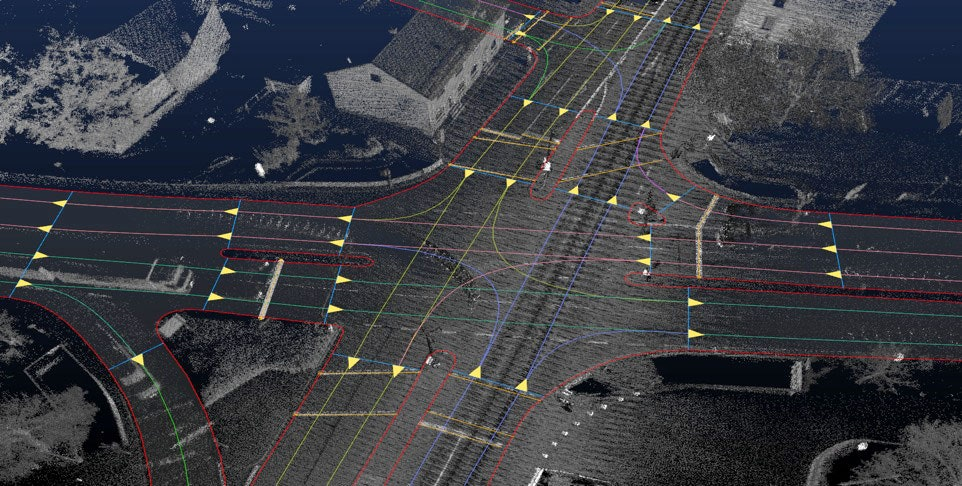
\includegraphics[scale=0.3]{required/HD-Map.jpg}
			\caption{Beispiel einer HD-map [Miller.2022]}			
		\end{figure}
	\end{frame}
	\begin{frame}{Implementierung: Datenverarbeitung}{Region of Interest}							\textbf{Anwendung}: Wissen über die Teststrecke als im Fahrzeug verfügbare HD-map \\		
		\textbf{Aufgabenstellung}: Begrenzung des Datensatzes auf Basis von 4 gegebenen Punkten $\hspace*{0.2em}^G\vspace*{-0.2em}P_{i}$ des globalen Koordinatensystems $G$ der Teststrecke
		\begin{figure}
			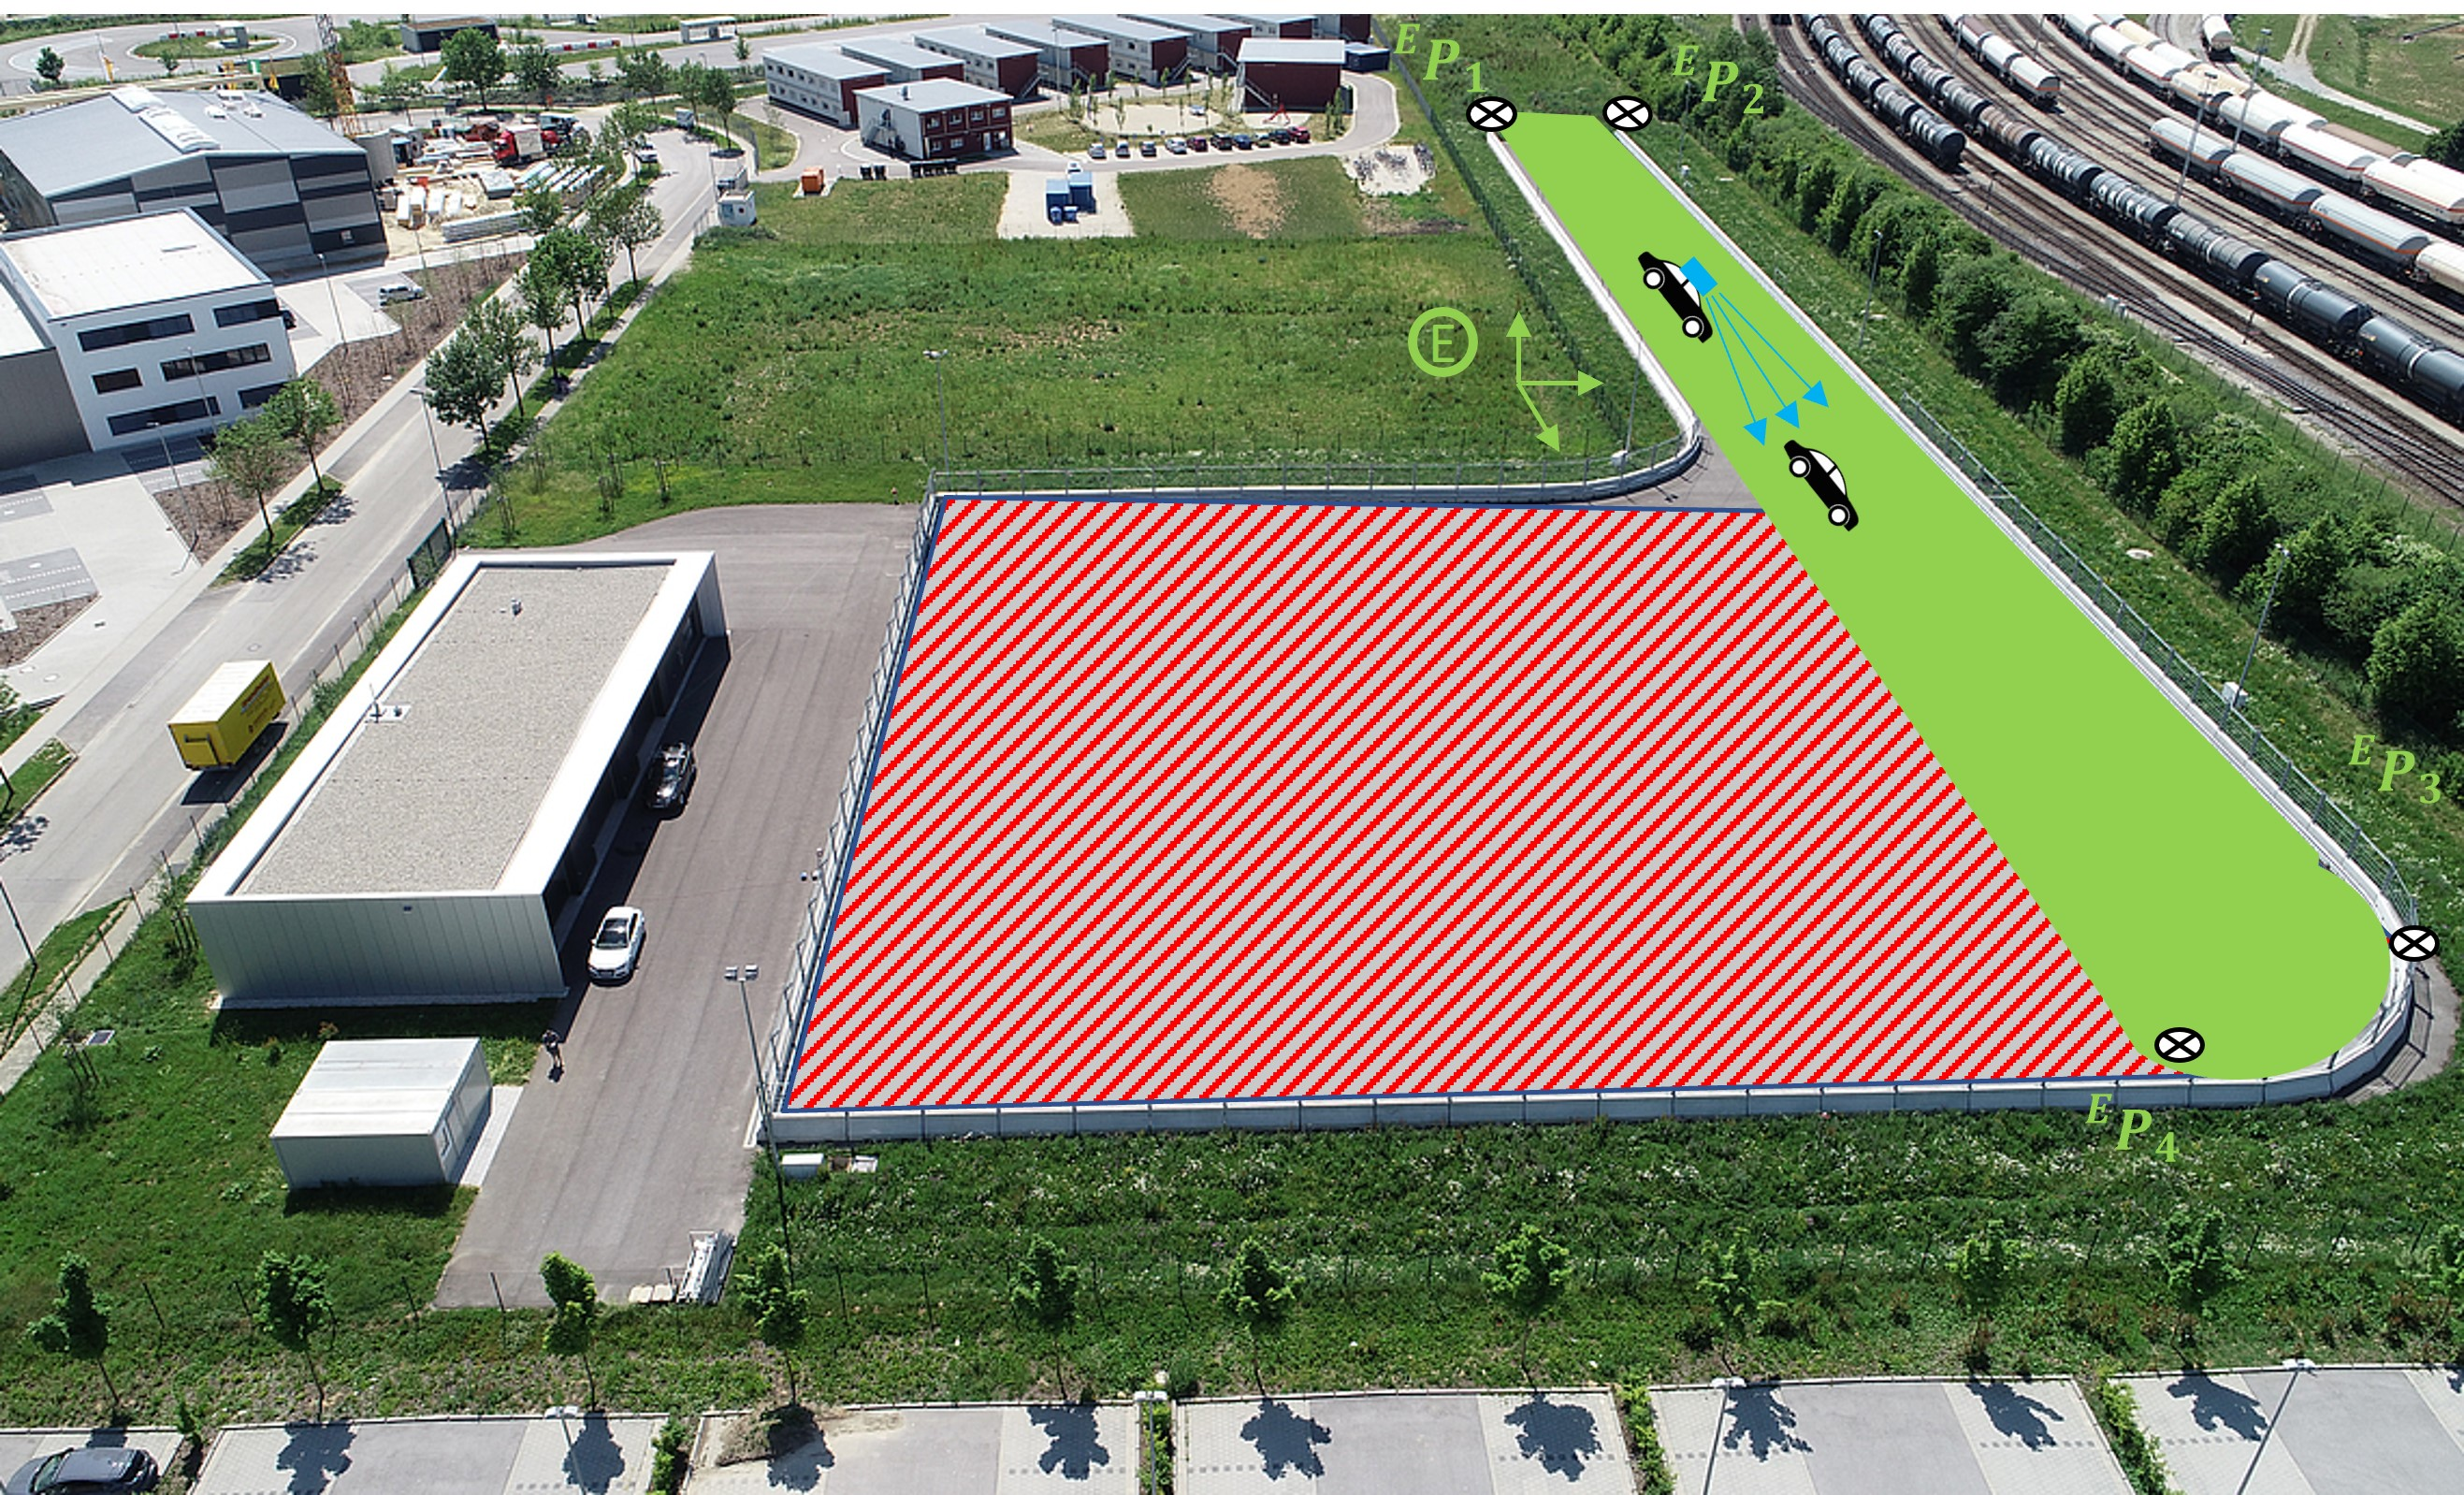
\includegraphics[scale=0.4]{required/ROI-Teststrecke.jpg}
		\end{figure}
	\end{frame}
	\begin{frame}{Datenverarbeitung}{Implementierung: Region of Interest}	
		\textbf{Gegeben:} 
		\begin{itemize}
			\item Punkte: $\hspace*{0.2em}^E\vspace*{-0.2em}P_{1}=(x,y,z)$, $\hspace*{0.2em}^E\vspace*{-0.2em}P_{2}=(x,y,z)$, $\hspace*{0.2em}^E\vspace*{-0.2em}P_{3}=(x,y,z)$, $\hspace*{0.2em}^E\vspace*{-0.2em}P_{4}=(x,y,z)$		
			\item Transformationsmatrizen: 
		\end{itemize}
		\textbf{Vorgehensweise:}
		\begin{enumerate}
			\item Transformation der LiDAR-Punkte $\hspace*{0.2em}^L\vspace*{-0.2em}P_{i}$ in das globale Koordinatensystem 
			\item Filterung aller Punkte mit Koordinaten $(x,y)$ außerhalb des durch die 4 Punkte $\hspace*{0.2em}^E\vspace*{-0.2em}P_{i}$ aufgespannten Bereichs
		\end{enumerate}
	\end{frame}
	\begin{frame}{Region of Interest}{Implementierungshinweise: Lokale Koordinatensysteme}
		\begin{figure}
			\centering
    		\begin{subfigure}[b]{0.4\textwidth}
				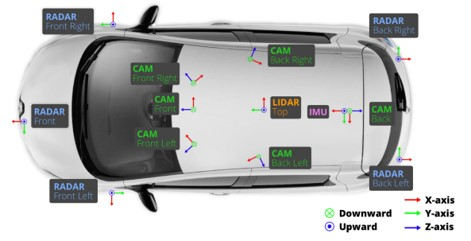
\includegraphics[scale=0.4]{required/Sensorkoordinatensysteme.jpg}
				\caption{Sensorkoordinatensysteme in nuScenes [Caesar.2020]}
        		\label{ROS}
   		 	\end{subfigure}
   		 	\vfill
    		\begin{subfigure}[b]{0.4\textwidth}
				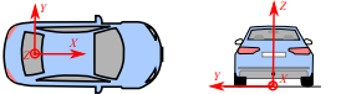
\includegraphics[scale=0.5]{required/Fahrzeugkoordinatensystem exterozeptiver Sensoren.jpg}
				\caption{Fahrzeugkoordinatensystem exterozeptiver Sensoren}
        		\label{ROS}
    		\end{subfigure}
    		\hspace{1.5 cm}
    		\begin{subfigure}[b]{0.4\textwidth}
				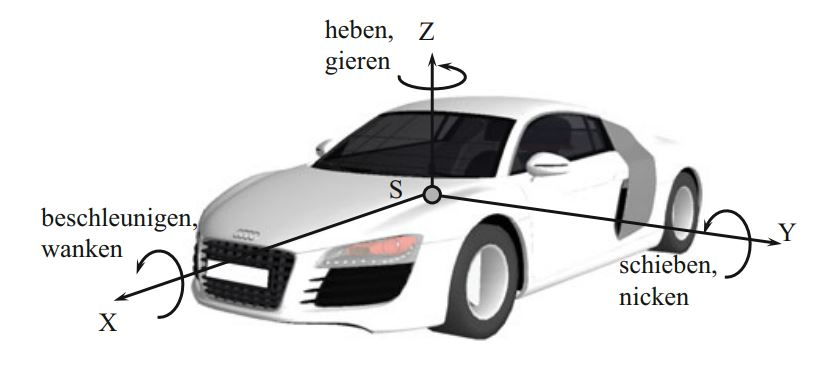
\includegraphics[scale=0.2]{required/Fahrzeugkoordinatensystem CoG.jpg}
				\caption{Fahrzeugkoordinatensystem der Fahrdynamikgleichungen [Breuer.2015]}
        		\label{ROS}
    		\end{subfigure}
		\end{figure}
		
	\end{frame}
	\begin{frame}{Region of Interest}{Implementierungshinweise: Lokale Koordinatensysteme}
		\begin{itemize}
			\item Zahlreiche Koordinatensysteme im Fahrzeug, die eine Betrachtung der Information aus verschiedenen Perspektive ermöglichen
			\item Zwischen den lokalen Koordinatensystemen des Fahrzeugs kann ein statischer Zusammenhang, analog einer Starrkörperbewegung, angenommen werden $\rightarrow$ Transformationsmatrizen sind zeitunabhängig
			\item Fahrzeugkoordinatensysteme sind bei der Berechnung zwingend zu beachten, da Sie den Variablen Bedeutung verleihen
			\item Beispiel einer Fahrdynamikgleichung:
			\begin{equation}
				\hspace*{0.2em}^V\vspace*{-0.2em}v_{x} = \frac{\delta}{\delta t}x \text{ gilt für } x =\hspace*{0.2em}^V\vspace*{-0.2em}x
			\end{equation}
					
		\end{itemize}
	\end{frame}
	\begin{frame}{Region of Interest}{Implementierungshinweise: Globale Koordinatensysteme}	
		\begin{figure}
			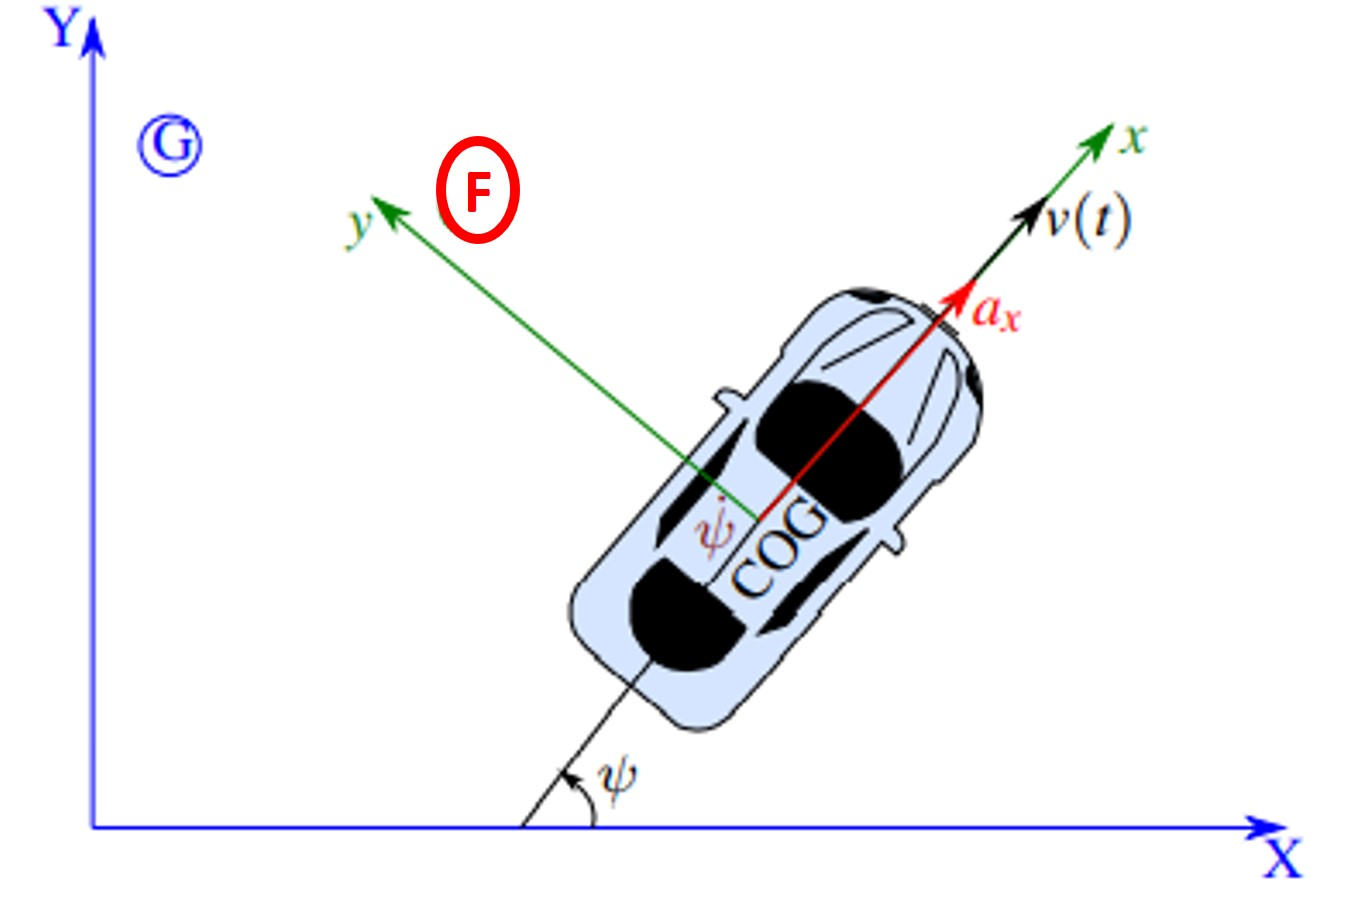
\includegraphics[scale=0.35]{required/Globales Koordinatensystem.jpg}
			\caption{Globales Koordinatensystem}
        	\label{Globales Koordinatensystem}
		\end{figure}
		\begin{itemize}
			\item Stationäres Referenzkoordinatensystem
			\item Ermöglicht die Beschreibung von Objekten relativ zu einem konstanten Koordinatensystem
			\item Transformationsmatrix von lokalem Fahrzeugkoordinatensystem zu globalem Koordinatensystem ist für instationäre Objekte zeitabhängig
		\end{itemize}					
	\end{frame}
	\begin{frame}{Region of Interest: Implementierungshinweise}{Anwendung auf das Szenario}
		\textbf{Nomenklatur:} 
		\begin{itemize}
			\item $\hspace*{0.2em}^E\vspace*{-0.2em}P$ : Punkt im globalen Koordinatensystem
			\item $\hspace*{0.2em}^L\vspace*{-0.2em}P$ : Punkt im LiDAR Koordinatensystem
			\item $\hspace*{0.2em}^V\vspace*{-0.2em}P$ : Punkt im Fahrzeugkoordinatensystem (CoG)
			\item $\hspace*{0.2em}^{S}\vspace*{-0.2em}P$ : Punkt im Fahrzeugkoordinatensystems der exterozeptiven Sensoren
		\end{itemize}
	\end{frame}
	\begin{frame}{Region of Interest}{Implementierungshinweise: Anwendung auf das Szenario}
		\begin{figure}
			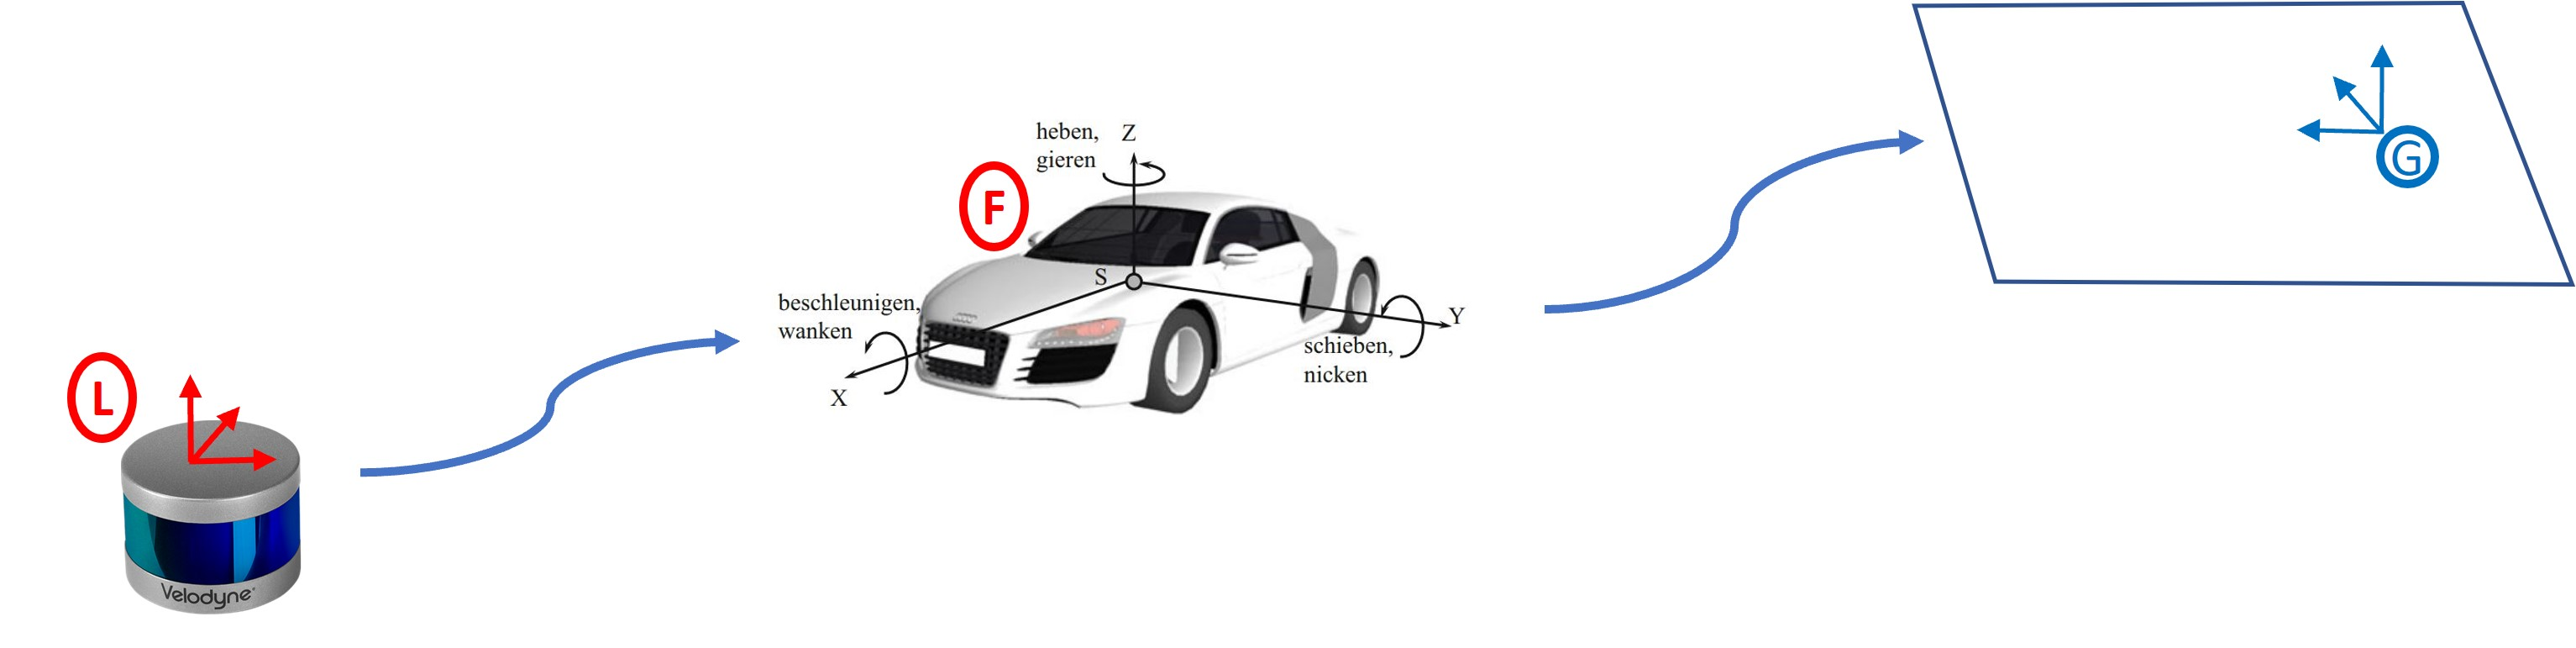
\includegraphics[scale=0.5]{required/Szenarioanwendung Koordinatentransformation.jpg}
			\caption{Anwendung der Koordinatentransformation auf das Szenario. Zusammengesetzt aus Abbildungen in [Breuer.2015] und [Velodyne.2020]}
        	\label{Globales Koordinatensystem}
       	\end{figure}
       	\footnotesize
       	\begin{itemize}
       		\item Innerhalb des Fahrzeug: statische Koordinatentransformation 
       		\item Zwischen Fahrzeug- und Erdkoordinatensystem: zeitabhängige Koordinatentransformation (Position des Fahrzeugs im globalen Koordinatensystem durch den ADMA-Sensor gegeben)
			\item Umsetzung mit tf-Modul aus ROS
       	\end{itemize}
	\end{frame}
	\begin{frame}{Region of Interest}{Implementierungshinweise: Transformation in ROS}	
		\footnotesize
		\textbf{Tutorial Links}
		\begin{enumerate}
			\item http://wiki.ros.org/tf/Tutorials
			\item http://wiki.ros.org/tf/Tutorials/Introduction\%20to\%20tf
			\item http://wiki.ros.org/tf2
			\item Youtube-Tutorial: https://www.youtube.com/watch?v=QyvHhY4Y\_Y8
		\end{enumerate}
		\textbf{Implementierung}
		\begin{itemize}
			\item Unterteilung in statische und dynamische (zeitabhängige) Transformatoren wird mit den jeweiligen Transformatoren umgesetzt
			\item Verwendung von rqt and rviz (see tutorial 2) um die Transformer zu visualisieren
		\end{itemize}

	\end{frame}
	\begin{frame}{Datenverarbeitung}{Implementierung: Ground Subtraction}
		\footnotesize
		\textbf{Motivation}
		\begin{itemize}
			\item LiDAR Sensor gibt zahlreiche Reflektionen der Fahrbahnoberfläche aus
			\item Diese Punkte gehören nicht zu den gesuchten Objekte und haben deswegen für die Objekterkennung keine Relevanz \\
		\end{itemize}
		\textbf{Ziele}
		\begin{itemize}
			\item Objektdetektionsalgorithmus muss Vernachlässigung von Reflektionen des Bodens nicht mehr erlernen
			\item Verkleinerung des Lösungsraums  
		\end{itemize}	
		\begin{figure}
			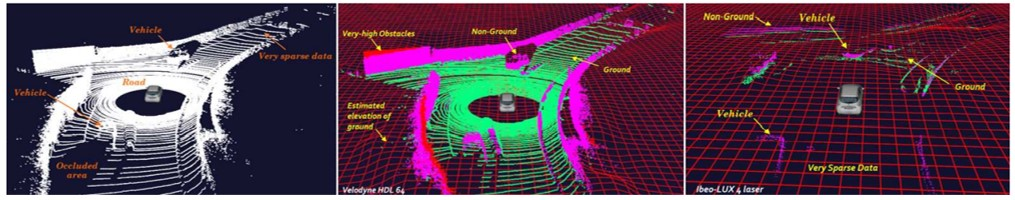
\includegraphics[scale=0.4]{required/Ground Subtraction.jpg}
			\caption{Beispiel Ground Subtraction [Rummelhard.2017]}
        	\label{Ground Subtraction}
       	\end{figure}
	\end{frame}
	\begin{frame}{Datenverarbeitung}{Implementierung: Ground Subtraction}
		\textbf{Anwendung:}
		\begin{itemize}
			\item Es wird eine ebene Fahrbahnoberfläche auf der Teststrecke angenommen
			\item Zur Vereinfachung wird die Eliminierung der Punkte der Fahrbahnoberfläche auf Basis Höhe $z$ durchgeführt
			\item Alternativen: RANSAC Algorithmus und weitere $\rightarrow$ weniger intuitiv, aber robuster			
		\end{itemize}
		\begin{figure}
			
\includegraphics[scale=0.5]{required/Ground Subtraction Implementierung.jpg} 
		\end{figure}
		\textbf{Aufgabenstellung:} Verkleinerung des Datensatzes um Punkte der Fahrbahnoberfläche: Bedingung $\hspace*{0.2em}^{EF}\vspace*{-0.2em}z \leq 0.01m$
	\end{frame}
	\begin{frame}{Datenverarbeitung}{Implementierung: Ground Subtraction}
		\footnotesize
		\textbf{Alternative:} RANSAC Algorithmus (hohe Robustheit, vor allem auch gegen Ausreißer)
		\begin{itemize}
			\item Iterativen Ansatz: Statt allen Messwerten gleichzeitig zu betrachten, wird nur eine zufällige Auswahl auswertet. Aus diesen Messwerten wird ein Modell erstellt und, auf Basis der Distanz zwischen Messwerten und Modell, die Anzahl der das Modell unterstütztenden Punkte gespeichert. Nach einer definierten Anzahl an Iterationen wird das beste Modell ermittelt
			\item Empfehlung: Verwendung einer existierenden High-Level Implementierung
		\end{itemize}

		\begin{figure}
			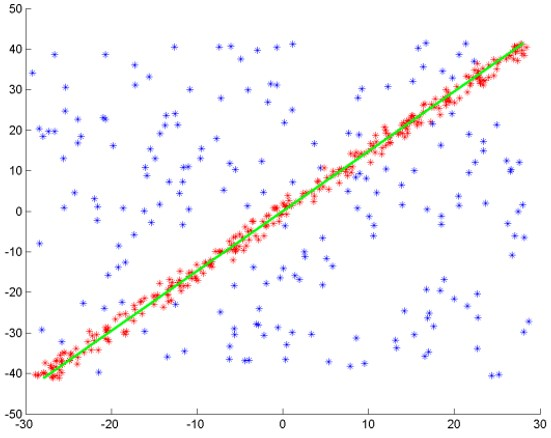
\includegraphics[scale=0.4]{required/RANSAC.jpg}
			\caption{Beispiel RANSAC-Algorithmus [RANSAC.2021]}
        	\label{Clustering}
		\end{figure}
	\end{frame}
	\begin{frame}{Datenverarbeitung}{Implementierung: Clustering}
		\small
		\textbf{Motivation:}
		\begin{itemize}
			\item Verwendung der \enquote{Ähnlichkeit} von Datenpunkten (bspw. Koordinaten), um zusammengehörende Punkte zu erkennen und zu segmentieren
			\item Ziel ist, die Struktur der Eingangsdaten zu lernen und eine automatische Segmentierung in Gruppen ähnlicher Datenpunkte vorzunehmen
		\end{itemize}
		\begin{figure}
			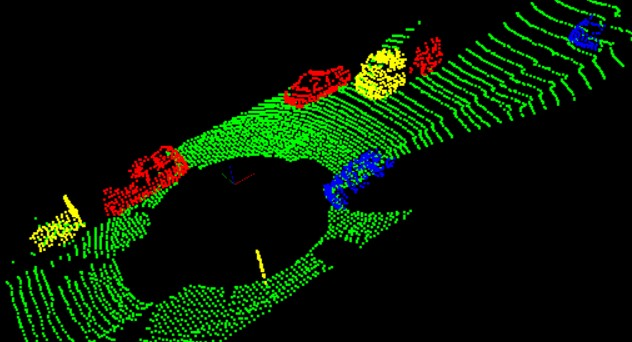
\includegraphics[scale=0.3]{required/Clustering.jpg}
			\caption{Beispiel Clustering [Hyin.2018]}
        	\label{Clustering}
		\end{figure}
	\end{frame}
	\begin{frame}{Datenverarbeitung}{Implementierung: Clustering}
		\textbf{Anwendung:} Angewandt auf unser Szenario bedeutet dies, das einzelne Gruppen LiDAR-Punkte zu Clustern vereint werden. Diese Punktwolken repräsentieren Objekte der Umgebung, wodurch final eine Lokalisierung des vorausfahrenden Fahrzeugs ermöglicht wird. \\
		\textbf{Aufgabenstellung:} Auf Basis des $k$-Means Clusteralgorithmus sollen die Datenpunkte des vorausfahrenden Autos gruppiert und segmentiert werden.
	\end{frame}		
	\begin{frame}{Datenverarbeitung}{Implementierungshinweise: Clustering}		
		\textbf{Allgemein:}
		\begin{itemize}
			\item Mehrere Optionen bei der Art der durchgeführten Clusteranalyse: partionierende, modellbasierte, hierachische, wahrscheinlichkeitsdichtebasierte, gitterbasierte Verfahren und Spectral Clustering
			\item In unserem Fall ($k$-Means Clustering): partionierendes Cluster-Verfahren, bei dem auf Basis der Merkmale der Datenpunkte ein Clustering vorgenommen wird. Jeder Punkt  $v_m$ des Datensatzes $\mathcal{D}$ wird eindeutig einem Cluster $C_1, ..., C_k$ zugewiesen. Das Cluster $C_K$ kann dementsprechend als Partion des Eingangsraums $\mathbb{R}^N$ interpretiert werden.
			\begin{equation}
				\mathcal{D} = \{v_1, ..., v_M \}
			\end{equation}
	\end{itemize}
	\end{frame}
	\begin{frame}{Clustering}{Implementierungshinweise: $k$-Means Algorithmus}
		\textbf{Beschreibung:} Aus einer Menge von ähnlichen Objekten wird eine vorher bekannte Anzahl von $k$ Clustern gebildet. Die Aufgabe wird gelöst, indem jeweils ein Repräsentant $c_k$ für jedes Cluster $C_k$ gesucht wird und zwar derart, dass alle Datenpunkte aus $\mathcal{D}$ nahe an ihrem jeweiligen Repräsentanten sind. \\
		\textbf{Umsetzung:} 
		\begin{itemize}
			\item Wenn $d(v_m, c_k)$ eine Distanz zwischen Eingangspunkt $v_m$ und Repräsentant des Clusters $c_k$ darstellt, so lässt sich die zu lösende Optimierungsaufgabe schreiben als
			\begin{equation}
				\{c_1, ..., c_k\}  = \underset{\{c_1',...,c_k'\}}{\mathrm{argmin}} \left\{\ \sum_{m=1}^M\ \underset{k=1, ...,K}{\mathrm{min}} d(v_m, c_k') \right\}\
			\end{equation}
			\item Diese Optimierungsaufgabe ist nicht konvex.
		\end{itemize}
 	\end{frame}
 	\begin{frame}{Clustering}{Implementierungshinweise: $k$-Means Algorithmus}
 		\begin{itemize}
 			\item Um die nicht konvexe Optimierungsaufgabe zu lösen wird ein iteratives Verfahren, der $k$-Means Algorithmus verwendet. Dieser findet ein lokales Optimum.
 			\item Nutzt man im $k$-Means Algorithmus als Distanzmaß die quadrierte Euklidische Distanz
 			\begin{equation}
 			 	d(v_m, c_k) = \lVert v_m - c_k \rVert_2 ^2
 			\end{equation}
 			\item Wird die Optimierungsaufgabe zu einer Minimierung der quadratischen Abweichungen von den Cluster-Schwerpunkten der Cluster $S_i$. Es kann von Clustering durch Varianzminimierung gesprochen werden. 
 			\begin{equation}
				J = \sum_{i=1}^k\ \sum_{x_j \in S_i}^{}\ \lVert v_m - c_k \rVert_2^2
			\end{equation}
 		\end{itemize}
 	\end{frame}
	\begin{frame}{Clustering}{Implementierungshinweise: $k$-Means Algorithmus}
		\textbf{Umsetzung LIoyd-Algorithmus:}
		\begin{itemize}
			\item 
			\begin{enumerate}
				\item Initialisierung: Wähle k zufällige Mittelwerte (Means): $m_1^{1},...,m_k^{1}$ aus dem Datensatz
				\item Zuordnung: Jedes Datenobjekt wird dem Cluster zugeordnet, bei dem die Cluster-Varianz am wenigsten erhöht wird
				\begin{equation}
					S_i^{t} = { x_j : \lVert x_j - m_i^{t} \rVert ^2 \text{ für alle } i^{*}=1, ..., k}
				\end{equation}
				\item Aktualisierung: Neuberechnung der Mittelpunkte der Cluster:
				\begin{equation}
					m_i^{t+1} = \frac{1}{|S_i^{(t)}|} \sum_{x_j \in S_i}^{}\ x_j
				\end{equation}
				\item Schritte 2-3 werden wiederholt, bis die Zentren $c_1, ..., c_k$ stabil sind, d. h. sich nicht mehr signifikant ändern.
			\end{enumerate}

		\end{itemize}
	\end{frame}
	\begin{frame}{$k$-Means-Algorithmus}{Vor- und Nachteile}
		\textbf{Vorteil:} 
		\begin{itemize}
			\item Leistungsfähigkeit (Komplexität $\mathcal{O}(kM)$ pro Iteration)
			\item Einfache Umsetzung, die lokales Minimum für die Optimierungsaufgabe liefert
			\item Eines der am häufigsten verwendeten Datensätze
		\end{itemize} 		
		\textbf{Nachteile:}		
		\begin{itemize}
			\item Gefundene Lösung hängt stark von der initialen, zufälligen Startpunkten ab
			\item Ausreißer in den Daten aus $\mathcal{D}$ beeinflussen , aufgrund der Mittelwertbildung für die Bestimmung der Clusterzentren, das finale Ergebnis stark
			\item Anzahl der Clusterzentren $k$ bereits im Voraus gewählt
		\end{itemize}
	\end{frame}
	\begin{frame}{Objektdefinition}{Bestimmung der Bounding Box}
		\footnotesize
		\begin{itemize}
			\item \textbf{Bounding Box:} Umschließt das Objekt und beschreibt dessen Position und Größe relativ zum Fahrzeug
			\item \textbf{Motivation:} Sensordatenverabeitung stellt of nur eine kompremierte Form der Information zur Verfügung. Dies ist z.B. eine Objektliste, die u. a. "bounding box"- Informationen enthalten kann. 
			\item \textbf{Vorgehen:} Bestimmung der Objektgrenzen auf Basis der segmentierten Objekt-LiDAR Punkte. Deren Koordinaten können für eine Bestimmung der Objektposition verwendet werden.
			\item \textbf{Implementierungshinweise:} Verwenden sie zur Vereinfachung den 2D Bird's eye view. Bestimmen Sie auf Basis der Punktkoordinaten das Objektzentrum und schätzen sie mit ihrem Wissen über die typische Größe eines Autos die bounding box. Mögliche Größe: $1.6 \text{ m} \times 3.9 \text{ m}$.
		\end{itemize}
		\begin{figure}
			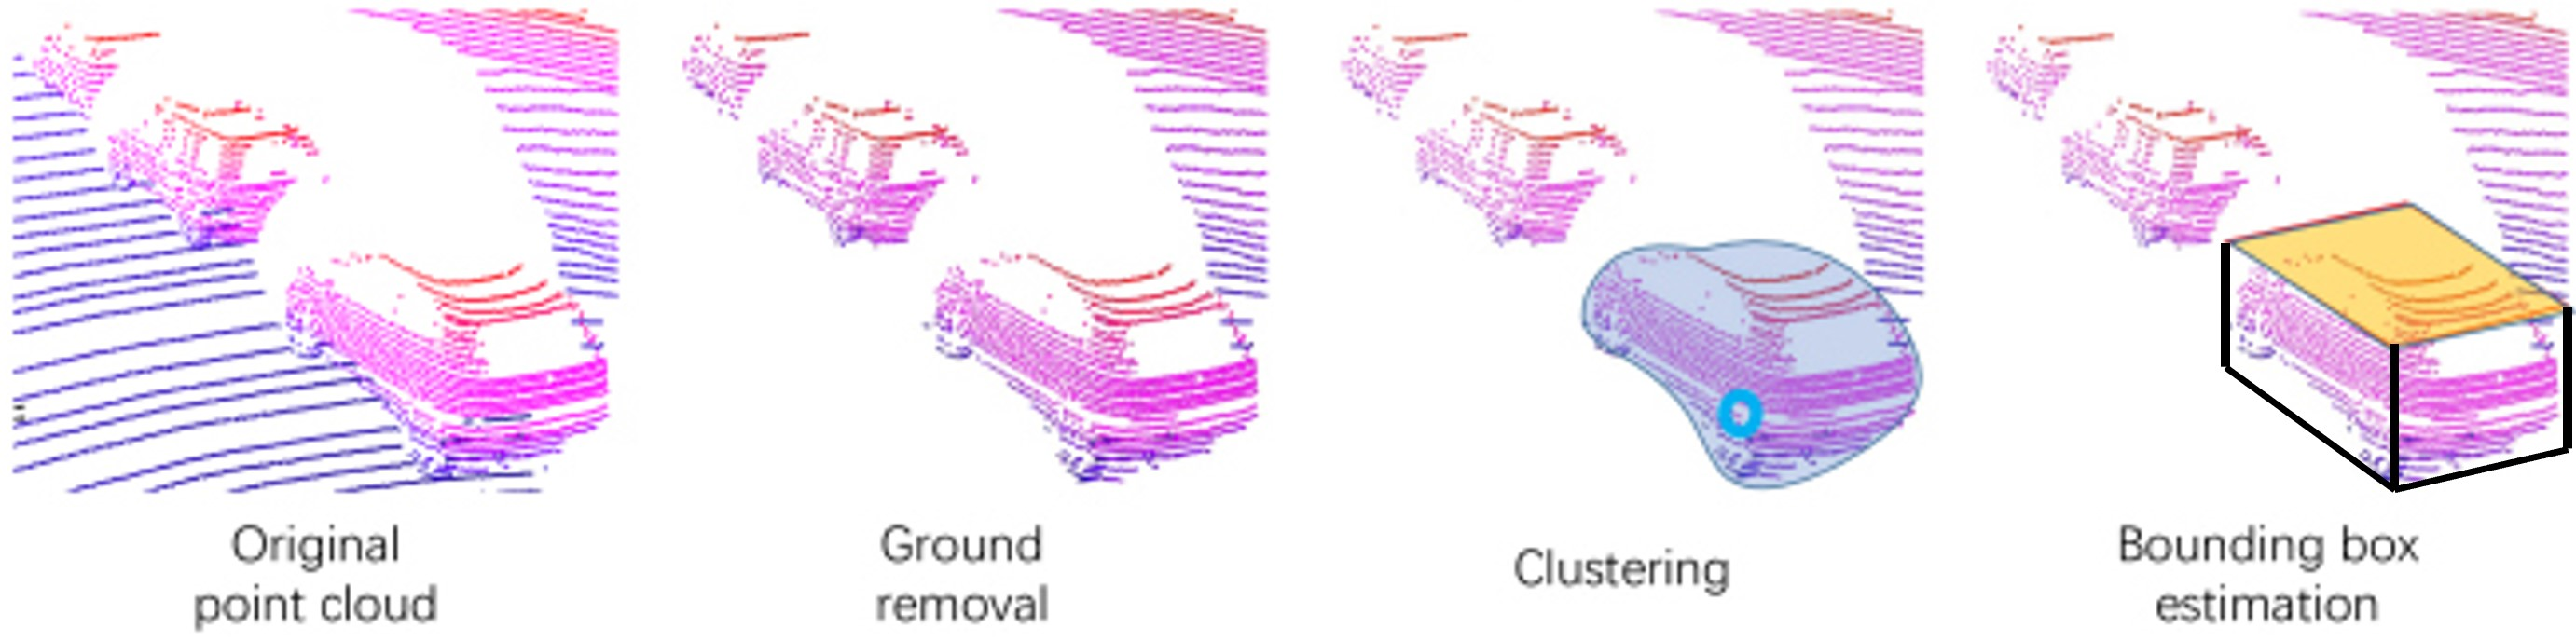
\includegraphics[scale=0.35]{required/Bounding_Box.jpg}
			\caption{Veranschaulichung der Bounding Box Bestimmung. Modifiziert von [Wang.2019]}
        	\label{Ground Subtraction}
       	\end{figure}
	\end{frame}
	\begin{frame}{KI-Algorithmus}{Erläuterung: Grundlagen des Maschinellen Lernens}
		Im Folgenden wird ein kurzer Einstieg in das Thema Maschinelles Lernen vermittelt. Der Fokus liegt auf einem oberflächlichen Verständnis für Begrifflichkeiten und Methoden. Es sei jedoch erwähnt, dass Maschinelles Lernen Mathematik und Statistik basiert, welche für ein tieferes Verständnis nötig ist, aber den Rahmen dieses Projektes übertreffen würde.
		Für einen tieferen Einstieg empfiehlt sich bspw.: 
		\begin{itemize}
			\item  Literatur: z.B. [Botsch.2020]
			\item Diverse Online-Quellen und Videos
			\item Studium im entsprechenden Bereich 
		\end{itemize}
	\end{frame}
	\begin{frame}{KI-Algorithmus}{Erläuterung: Grundlagen des Maschinellen Lernens}
		\footnotesize
		\textbf{Allgemein:} Der Begriff Maschinelles Lernen fasst Methoden der Signalverarbeitung zusammen, die statistische Zusammenhänge in Daten mit Hilfe von Computern finden und damit in der Lage sind, zukünftige Daten vorherzusagen. Man spricht auch von der künstlichen Generierung von Wissen aus Erfahrung. Das maschinelle Lernen beruht auf der mathematischen Statistik und beschäftigt sich mit dem „Lernen“ aus Daten, d. h. mit dem Finden von Gesetzmäßigkeiten in den Daten\\
		\begin{figure}
			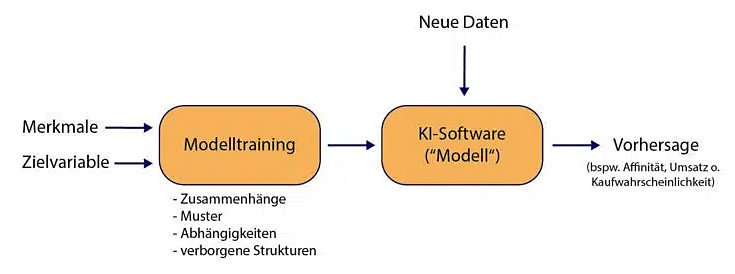
\includegraphics[scale=0.5]{required/ML_Einfuhrung.jpg}
			\caption{Grundkonzept des maschinellen Lernens [Wuttke.2020]}
        	\label{Ground Subtraction}
       	\end{figure}

	\end{frame}
	\begin{frame}{KI-Algorithmus}{Erläuterung: Grundlagen des Maschinellen Lernens}
		Maschinelles Lernen ist ...
		\begin{itemize}
			\item ein Teilbereich der künstlichen Intelligenz
			\item zunehmend relevant in allen Ingenieurswissenschaften, da die Rechenleistung und verfügbare Datenmenge in den letzten Jahren stark zugenommen hat
			\item fähig zahlreiche komplexe praktische Anwendungen erfolgreich zu bearbeiten
	\end{itemize}		
		Die Arbeitsschritte lassen sich grob folgender Maßen zusammenfassen:
		\begin{enumerate}
			\item Definition der Ziele
			\item Vorbereitung der Daten
			\item Lernphase
			\item Interpretation der Ergebnisse
			\item Nutzung in einer praktischen Anwendung
		\end{enumerate}
	\end{frame}
    \begin{frame}{KI-Algorithmus}{Erläuterung: Grundlagen des Maschinellen Lernens}
		\begin{figure}
			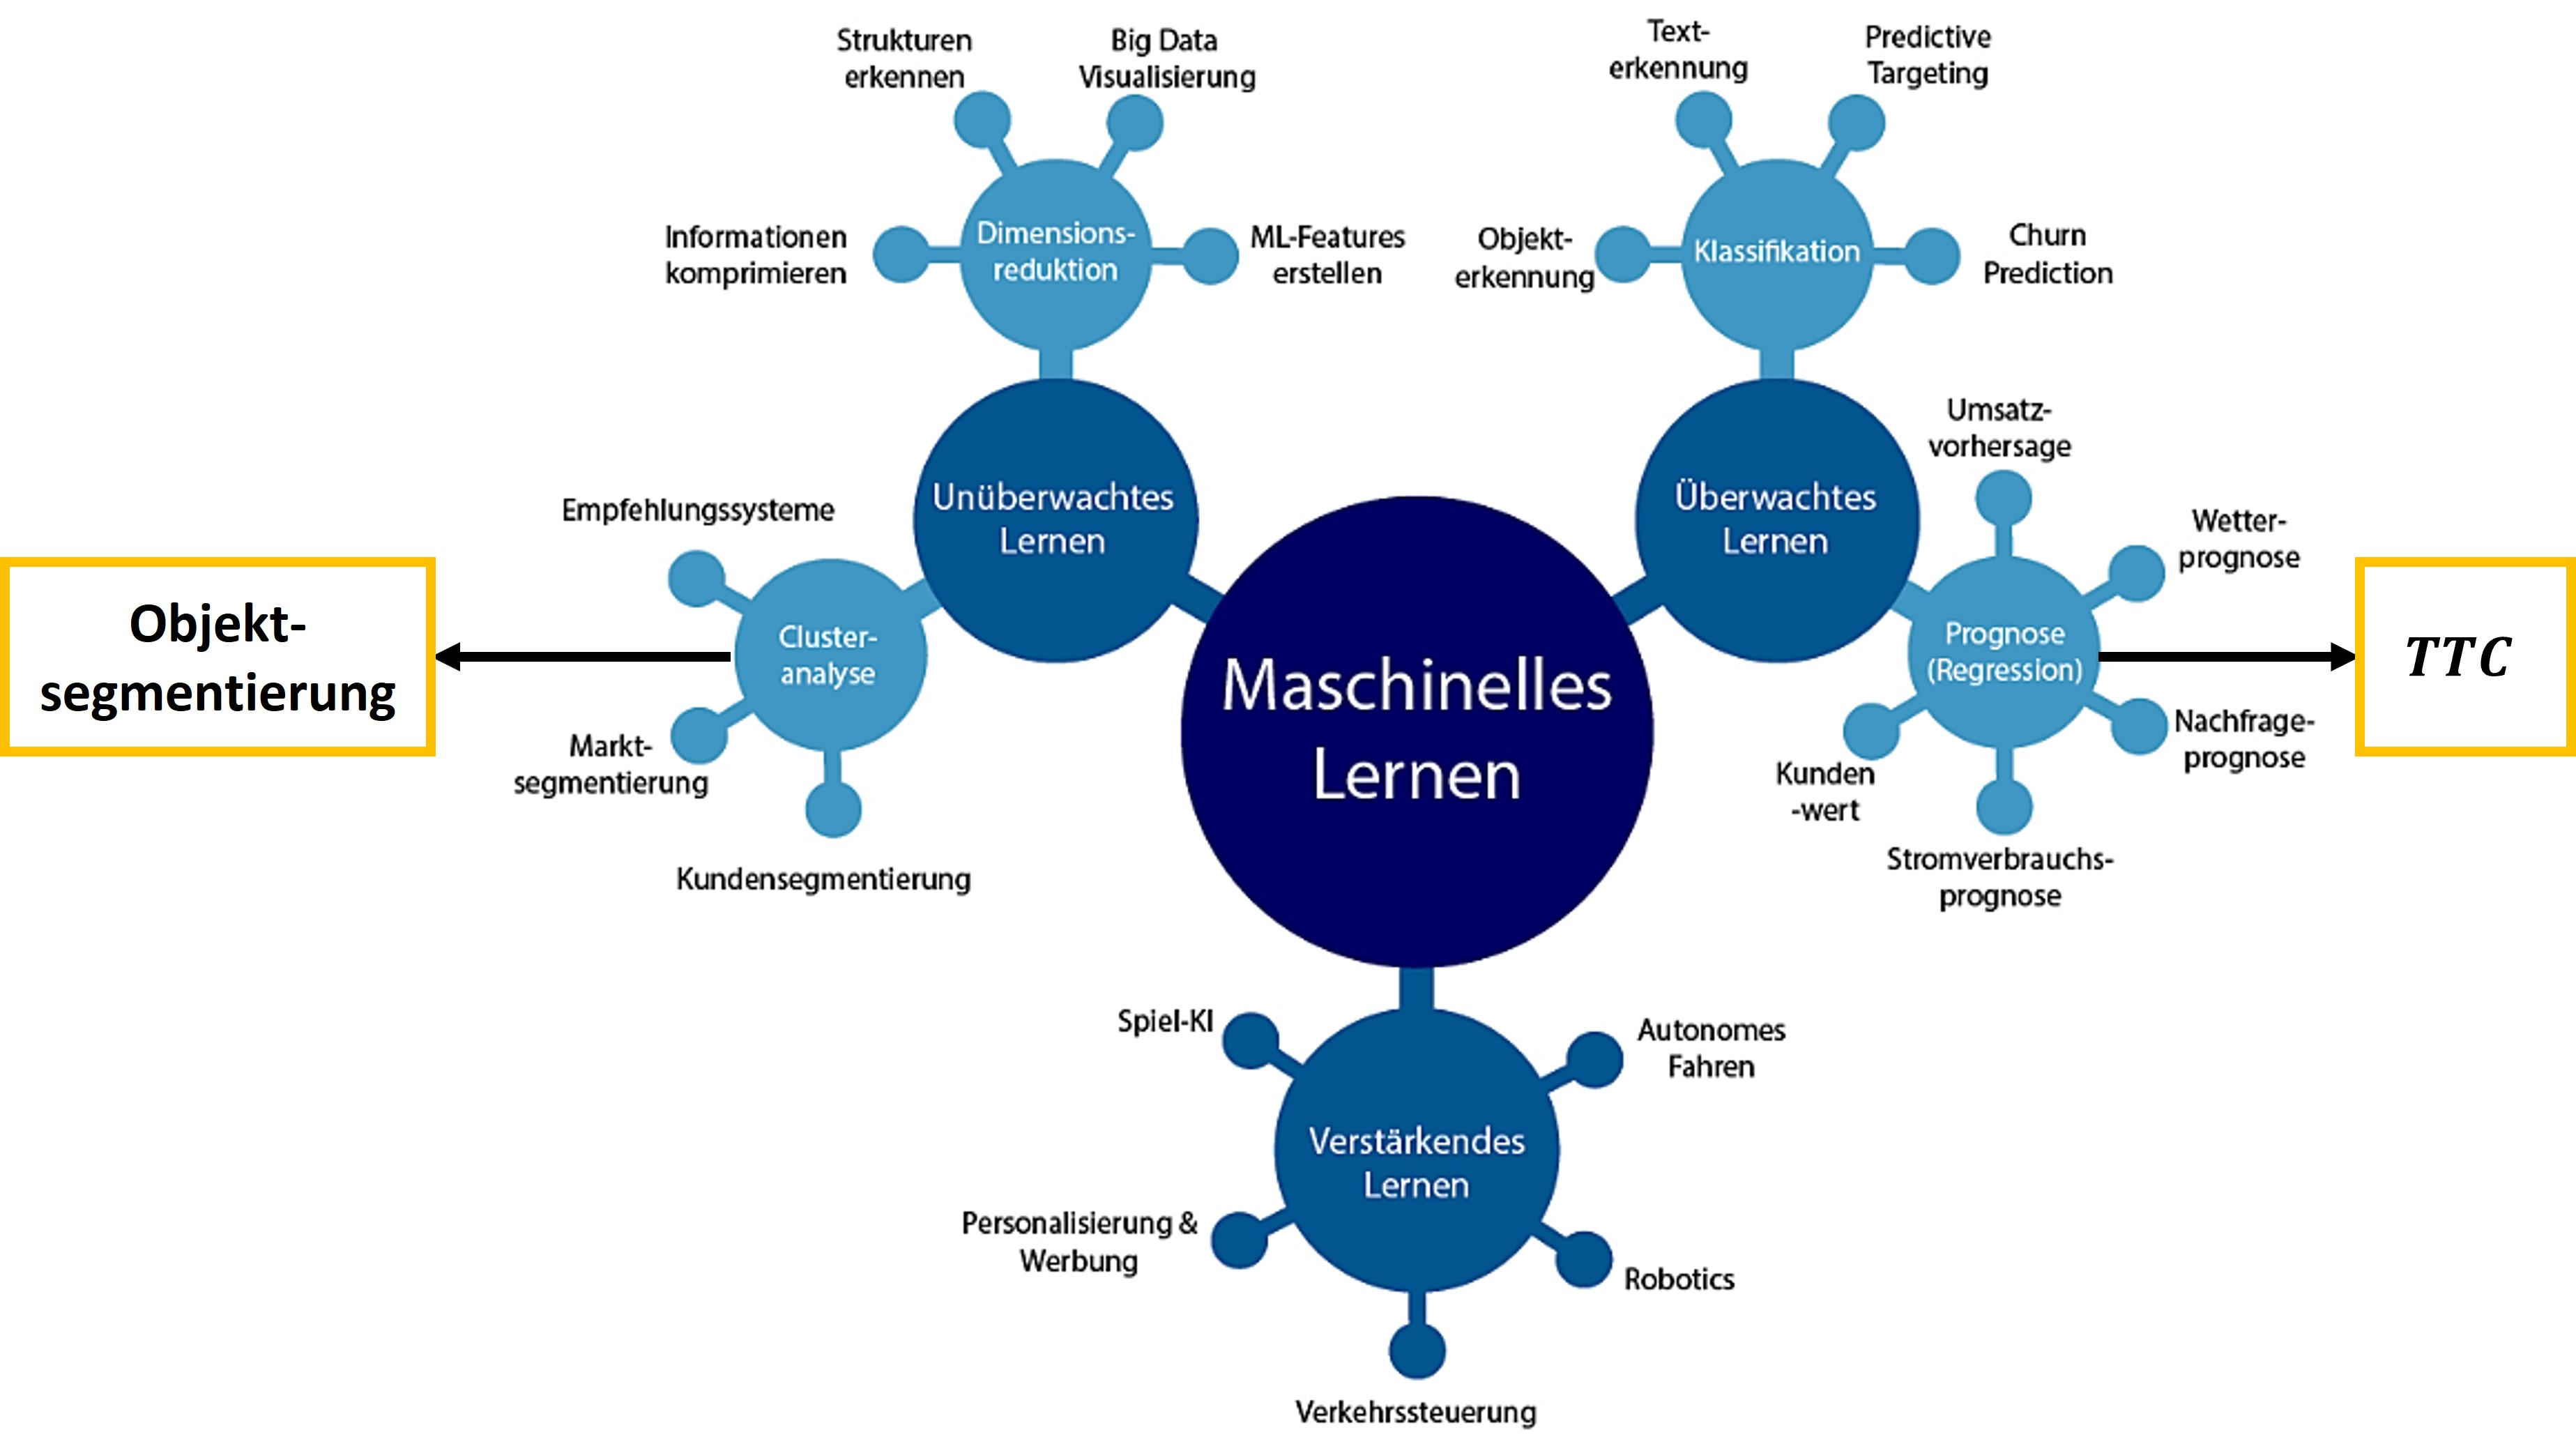
\includegraphics[scale=0.4]{required/Bereiche_Machine_Learning.jpg}
			\caption{Anwendungsgebiete des maschinellen Lernens[Wuttke.2020]}
        	\label{Ground Subtraction}
       	\end{figure}
     
    \end{frame}
    \begin{frame}{KI-Algorithmus}{Erläuterung: Grundlagen des Maschinellen Lernens}
		\vspace{1cm}       	
       	\textbf{Hinweis:} Der bereits angewandte $k$-Means-Algorithmus entspricht damit Maschinellem Lernen. Die Art wird des unüberwachten Lernens (eng. Unsupervised Learning) genannt. Bei dieser lernt Algorithmus allein aus den Eingängen, es gibt keine zugehörigen Ausgangsdaten. Ziel ist es, die Struktur in den Eingangsdaten zu lernen und ein Modell dafür zu erstellen.
	\end{frame}
	\begin{frame}{KI-Algorithmus}{Erläuterung: Grundlagen des Maschinellen Lernens}
		\small	
		\textbf{Überwachtes Lernen} (engl. Supervised Learning)	
		\footnotesize
		\begin{itemize}
			\item Eine Art des maschinellen Lernens (Andere: Unsupervised Learning, Semi-Supervised Learning, Reinforcement Learning)
			\item Ein Algorithmus lernt aus Beispielen von Eingängen und Ausgängen, d. h. es sind Eingangsdaten und zugehörige Ausgangsdaten (label)
für das Lernen vorhanden. Ziel ist es, Vorhersagen für neue, unbekannte Eingangsdaten zu machen.
		\end{itemize}
		\begin{figure}
			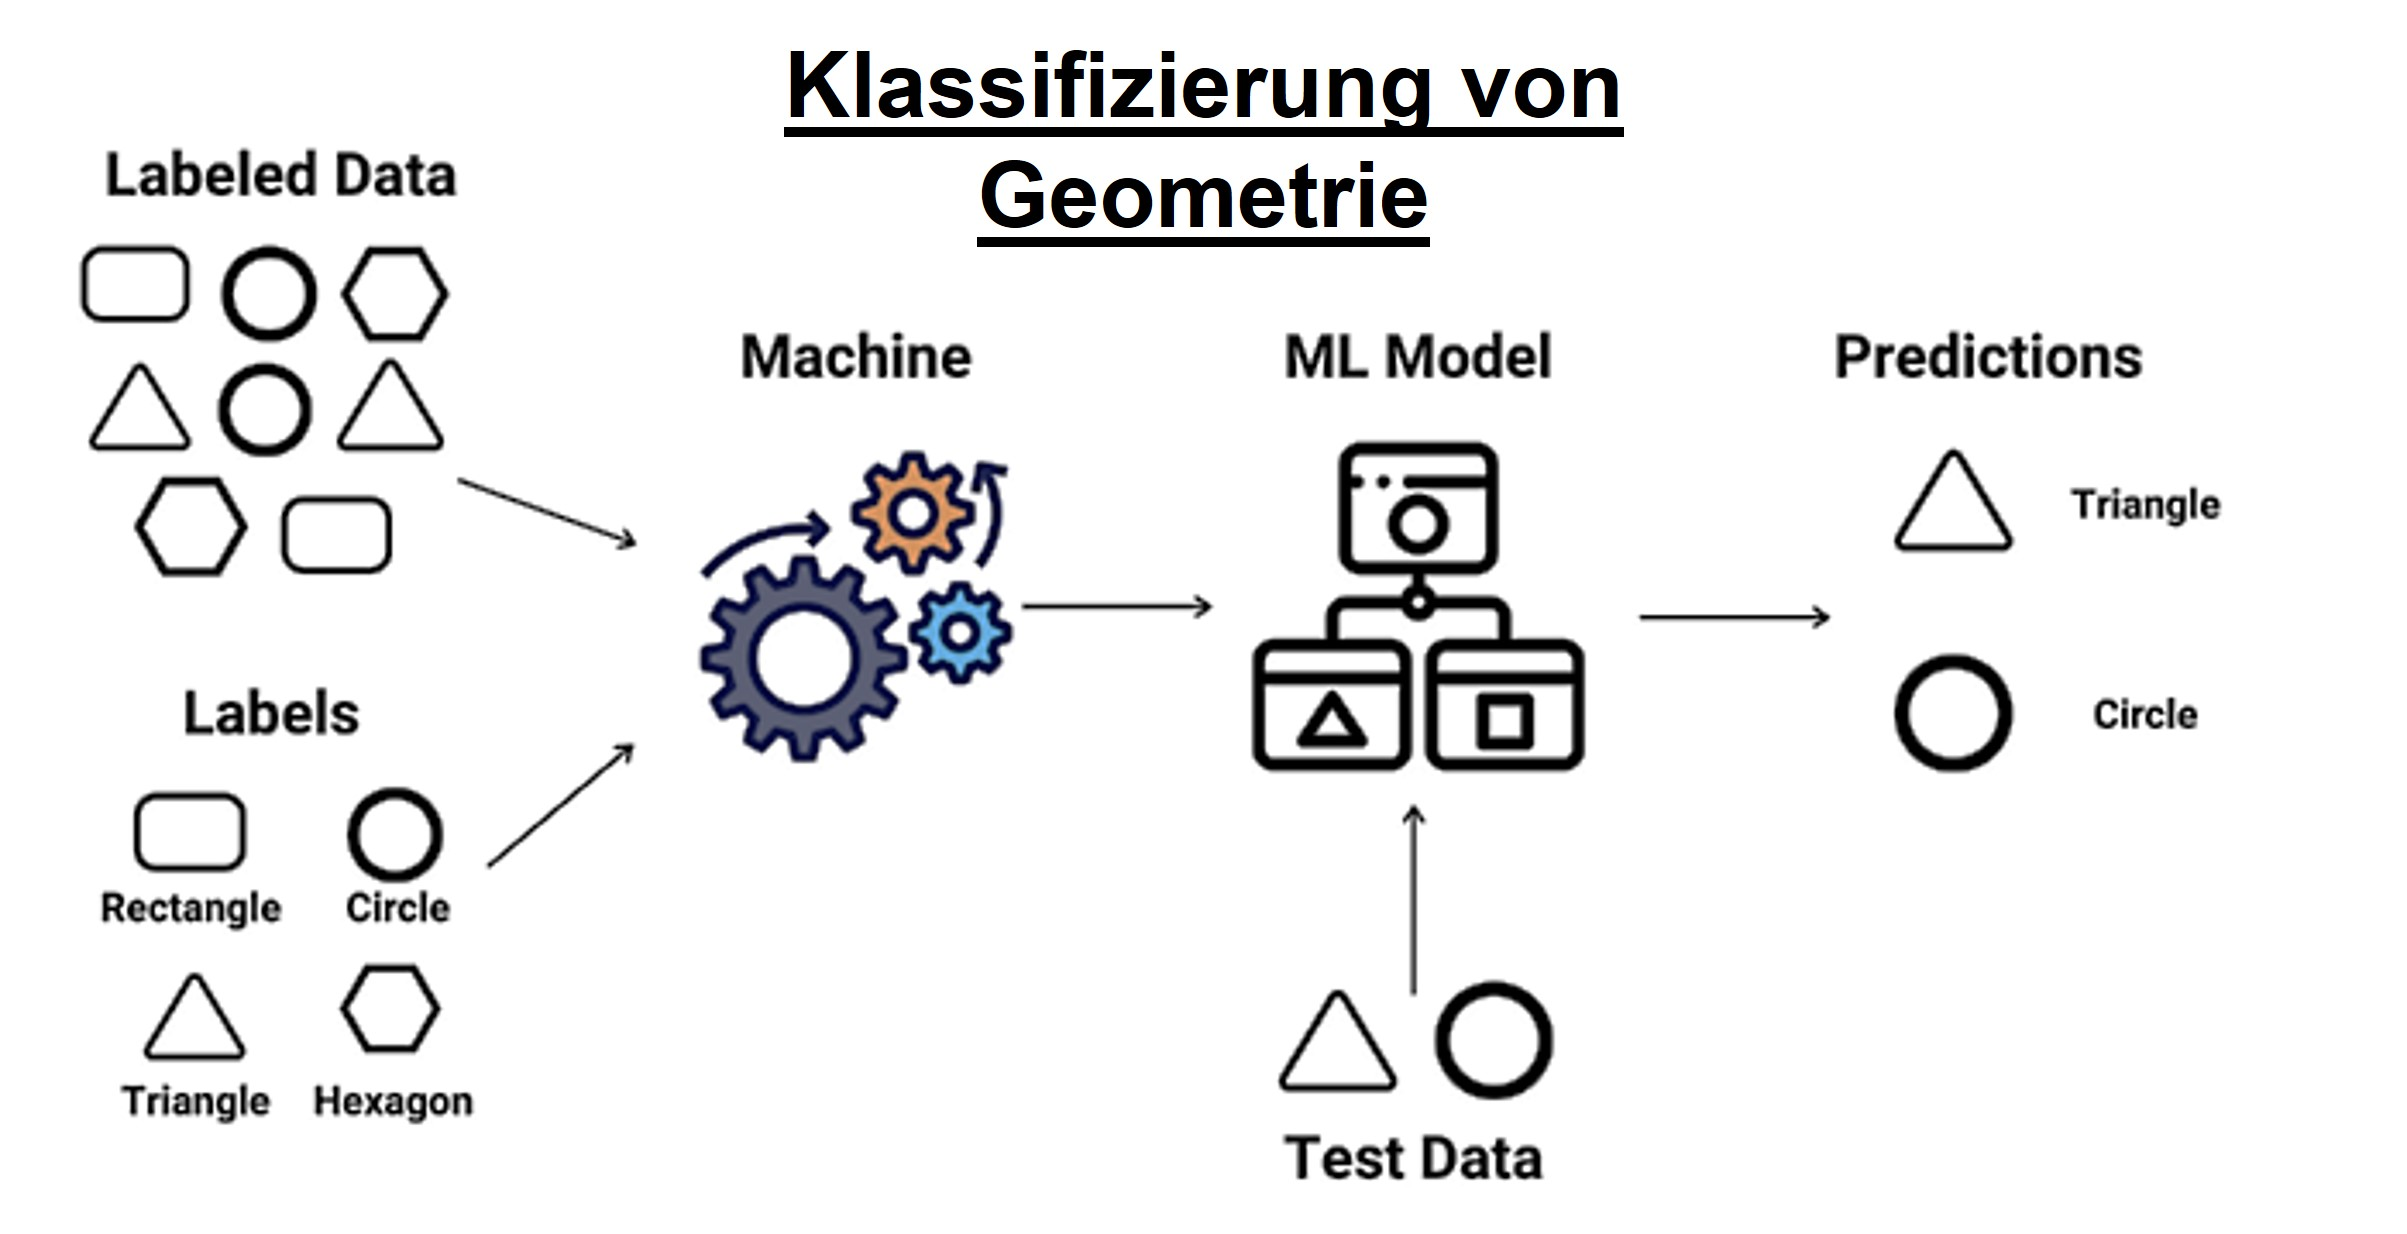
\includegraphics[scale=0.3]{required/supervised_learning.jpg}
			\caption{Beispiel für Überwachtes Lernen [Kozan.2021]}
        	\label{Ground Subtraction}
       	\end{figure}
	\end{frame}

	\begin{frame}{KI-Algorithmus}{Erläuterung: Grundlagen des Maschinellen Lernens}
		\begin{itemize}
			\item \textbf{Ziel:} Algorithmus zur Bestimmung einer beschreibenden Größe eines Systems, basierend auf im Vorfeld beobachteten Merkmalen dieses Systems, zu finden. Der Algorithmus soll dann auf Fälle angewandt werden, bei denen die Werte der zu beschreibenden Größe unbekannt sind
			\item Wenn pro Beobachtung $N$ Merkmale vorliegen, so werden diese im Vektor \textbf{x} zusammengefasst
			\begin{equation}
				\textbf{x} = [x_1,..., x_{N}]^{T} \in \mathbb{R}
			\end{equation}
			\item Die zu beschreibende Größe wird mit \textbf{y} notiert, die durch den Algorithmus berechnete mit $\hat{\textbf{y}} = f(\textbf{x})$.
		\end{itemize}	
	\end{frame}
	\begin{frame}{KI-Algorithmus}{Erläuterung: Grundlagen des Maschinellen Lernens}
		\textbf{Regression}	
		\begin{itemize}
			\item Falls $\textbf{y}$ kontinuierliche Werte annimmt, also $\textbf{y} \in \mathbb{R}$, werden die Eingangswerte \textbf{x} auf eine Ausgabe $\hat{\textbf{y}}$ regressiert 
			\item Ziel ist, dass die tatsächliche Lösung $\textbf{y}$ möglichst gut durch $\hat{\textbf{y}} $ approximiert wird.
		\end{itemize}			
		\begin{figure}
			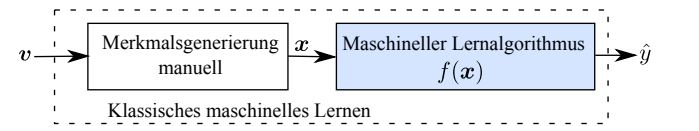
\includegraphics[scale=0.7]{required/Machine Learning.jpg}
			\caption{Regression als Algorithmus des klassischen maschinellen Lernens}
        	\label{Machine Learning}
		\end{figure}
	\end{frame}
	\begin{frame}{KI-Algorithmus}{Erläuterung: Grundlagen des Maschinellen Lernens}
		\footnotesize
		\textbf{Training: } 		
		\scriptsize	
		\begin{itemize}
			\item Das Lernen basiert auf einer Verlustfunktion und dessen Gradienten. Diese erfasst den Unterschied zwischen dem Ausgang $\hat{\textbf{y}}$ und dem Zielwert $y$ quantitativ.
			\item Das Ziel des Trainings ist damit, die Funktion $f$ zu finden, bei der dieser Verlust möglichst gering ist. 
			\item Eine häufig verwendete quadratische Verlustfunktion lautet beispielsweise:
			\begin{equation}
				\mathcal{L}(\textbf{y}, f(\textbf{x})) = (\textbf{y} - f(\textbf{x}))^{2}
			\end{equation}
		\end{itemize}	
		\begin{figure}
			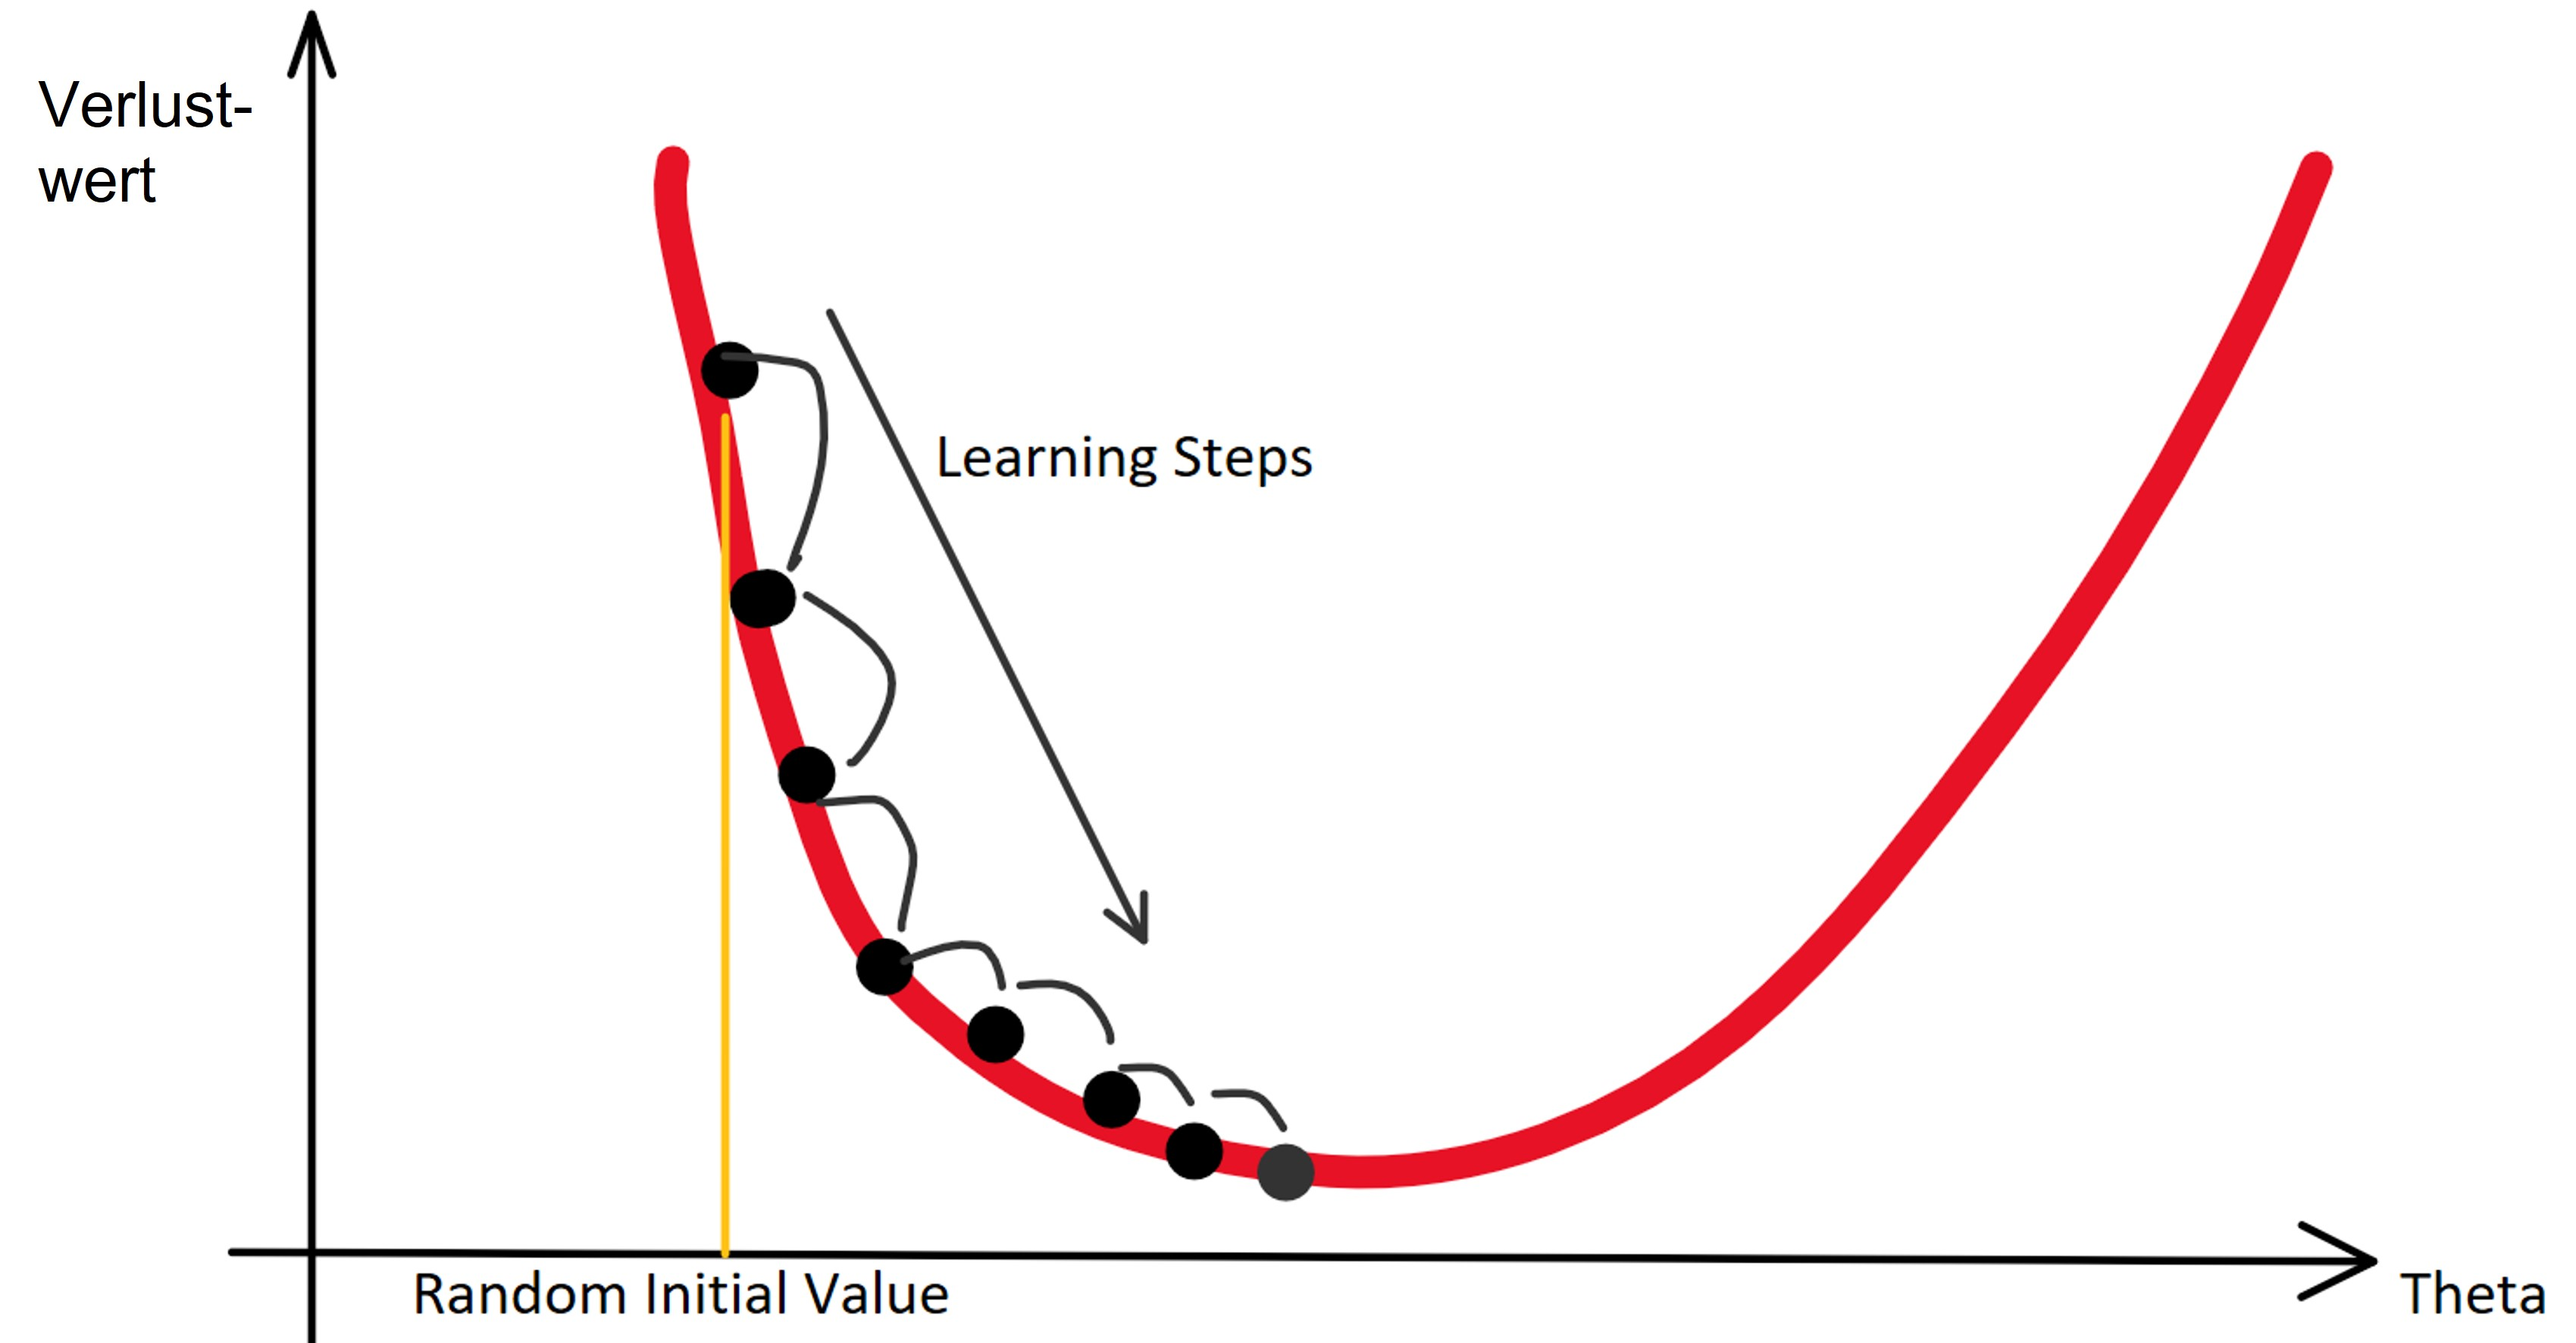
\includegraphics[scale=0.2]{required/Loss_function.jpg}
			\caption{\scriptsize Gradientenabstiegsverfahren [Aunkofer.2019]}
        	\label{Machine Learning}
		\end{figure}			
	\end{frame}
	\begin{frame}{KI-Algorithmus}{Erläuterung: Grundlagen des Maschinellen Lernens}
		\small		
		\textbf{Funktion f(x):}
		\begin{itemize}
			\item Je komplizierter die Funktion, desto mehr Parameter müssen im Training erlernt werden. Eine simple Beispielfunktion ist die lineare Gleichung. Diese wird im Folgenden noch genauer erklärt.
			\item Gleichzeitig gilt aber auch: Je mehr Parameter erlernt werden können, desto kompliziertere Zusammenhänge können auch dargestellt werden. 
			\item Die Komplexität der Funktion spielt eine entscheidende Rolle für Over- bzw. Underfitting
		\end{itemize}
	\end{frame}
	\begin{frame}{KI-Algorithmus}{Erläuterung: Grundlagen des Maschinellen Lernens}
		\footnotesize		
		\textbf{Over- und Underfitting:}	
		\begin{itemize}
			\item Beachte: Auch der verwendete Trainingsdatensatz unterliegt der Statistik (Welcher Teil der Realität wird dargestellt?, Messfehler?, Rauschen?, etc.)		
			\item Bei zu hoher Freiheit, kann der Verlust im Training sehr gering werden, obwohl der Algorithmus für neue, unbekannte Daten weniger gut approximieren würde. ist. Grund dafür ist, dass der Algorithmus sich zu stark an den eingeschränkten Trainingsdatensatz anpasst. Man spricht von Overfitting.
			\item Bei zu geringer Freiheit, kann die Funktion den geforderten Datensatz nicht darstellen. Man spricht von Underfittng.
		\end{itemize}
		\begin{figure}
			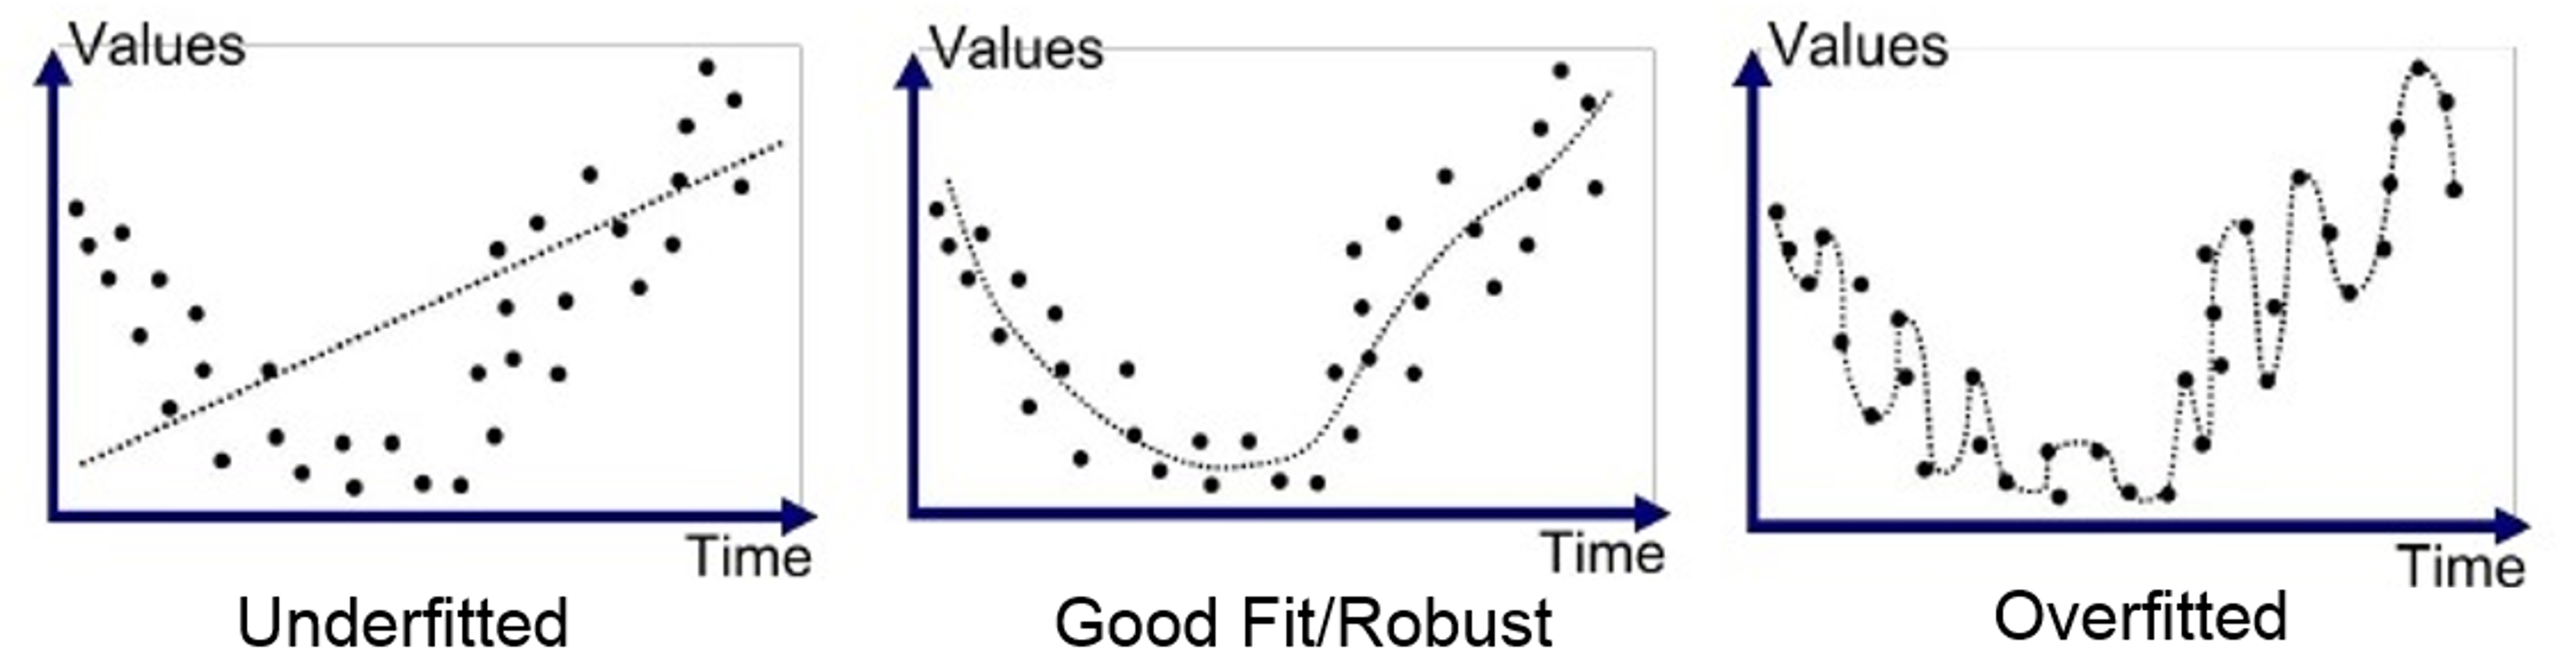
\includegraphics[scale=0.25]{required/Over and Underfitting.png}
			\caption{\scriptsize Beispiel für Overfitting und Underfitting [Bhande.2018]}
        	\label{Over and Underfitting}
		\end{figure}
	\end{frame}
	\begin{frame}{KI-Algorithmus}{Erläuterung: Grundlagen des Maschinellen Lernens}
		\textbf{Umgang mit großen Datenmengen:}
		\begin{itemize}
			\item Falls $M$, die Anzahl der Datenpunkte, sehr groß wird, kann es sinnvoll sein den Datensatz im Training in sogenannte Batches aufzuteilen und sich über ein Gradientenabstiegsverfahren sequentiell der Lösung anzunähern.
			\begin{equation}
				\Theta ^{(l+1)} = \theta ^{(l)} - \alpha \frac{\delta}{\delta \theta} \Bigl(\mathcal{L} (y_m, f_{\theta} (x_m))\Bigr) \Big| _{\theta = \theta^{(l)}}
			\end{equation}
			\item[] Dabei ist $l$ der Index der Iteration und $\alpha$ die sogenannte Lernrate, die die Schrittweite pro Iteration festlegt.
			\item Nutzt man für die Aktualisierung der Parameter den gesamten Datensatz $\mathcal{D}$, so nennt man dies eine Epoche.
		\end{itemize}
	\end{frame}
	\begin{frame}{KI-Algorithmus}{Erläuterung: Grundlagen des Maschinellen Lernens}
		\textbf{Normierung}
		\begin{itemize}
			\item Bei der Minimierung des quadratischen Fehlers haben Merkmale $x_n$, deren Wertebereich auch Zahlen mit großem Betrag enthält, einen größeren Einfluss auf die Lösung, als Merkmale, deren Wertebereich nur Zahlen mit kleinem Betrag besteht.
			\item Um dies zu neutralisieren, werden die Wertebereiche aller Merkmale auf das Intervall [0, 1] abgebildet
			\begin{equation}
				x_{n,m}^{\text{norm}} = \frac{x_{n,m} - x_{n,\text{min}}}{x_{n,\text{max}} - x_{n,\text{min}}}
			\end{equation}
		\end{itemize}
	\end{frame}
	\begin{frame}{KI-Algorithmus}{Erläuterung: Ermittlung der kritischen Zeit}
		\textbf{Motivation}
		\begin{itemize}
			\item Die Berechnung der kritischen Zeit ist auch aus Fahrdynamikgleichungen ableitbar und setzt deswegen keine Notwendigkeit für KI-Algorithmen voraus.
			\item Die dadurch gegebene Intuition für das Ergebnis ermöglicht aber ein gutes Verständnis für die Möglichkeiten und Grenzen von KI-Algorithmen.
			\item Ziel ist die kritische Zeit bis zum Auffahrunfall zu berechnen, um z. B. eine Notbremsung zu entwerfen
		\end{itemize}
	\end{frame}
	\begin{frame}{KI-Algorithmus}{Erläuterung: Ermittlung der kritischen Zeit}
		Ein Maß für die Kritikalität eines Verkehrsszenarios ist die sogenannte \textbf{\enquote{Time-To-Collision} (TTC)} \\ 
		\textbf{Erläuterung:}
		\begin{itemize}
			\item Je kleiner der Wert der TTC, desto kritischer das Szenario
			\item Für Auffahrunfälle: TTC kann aus der Distanz $d$ der beiden Fahrzeuge und der relativen Geschwindigkeit $v_{x,\text{rel}}$ bestimmt werden
			\begin{equation}
				TTC = 
				\begin{cases}
					\frac{d}{|v_{\text{x,\text{rel}}}|} \text{ für } v_{x,\text{rel}}<0 \\
					\tau \text{ für } v_{x,\text{rel}} \geq 0 \text{,}
				\end{cases}
			\end{equation}
			\item[] wobei $\tau$ einen großen Wert besitzt, der indiziert, dass das Szenario unkritisch ist.
		\end{itemize}			
	\end{frame}
	\begin{frame}{KI-Algorithmus}{Implementierung: lineare Regression}
		\begin{enumerate}
			\item Generieren Sie einen Datensatz $\mathcal{D}_{train}$ mit den Eingangsvektoren $x_m$, der die Distanz und relativ Geschwindigkeit zwischen Ego- und vorausfahrendem Fahrzeug enthält. Erzeugen sie zudem das zugehörige Label, die kritische Zeit bis zur Kollision. Damit sind die Zufallsvariablen für Ein- und Ausgang:
		\begin{equation}
			x = 			
			\begin{bmatrix}
				d & v_{x,\text{rel}}
			\end{bmatrix}
			^{\text{T}} \in \mathbb{R} 
			\hspace{0.2 cm}
			\text{und}
			\hspace{0.2 cm}			
			y = TTC \in \mathbb{R}
		\end{equation}
			\item[] Vorgaben bei der Erzeugung des Trainingsdatensatzes $\mathcal{D}_{\text{train}}$:
			\begin{itemize}
				\item Distanz $d$: Schrittweite $1m$; Intervall $[1m, 30m]$ 
				\item Relativgeschwindigkeit $v_{x,\text{rel}}$: Schrittweite $5 km/h$; Intervall $[-60 km/h, -5 km/h]$
				\item $\tau = 60s$
			\end{itemize}			 
		\end{enumerate}
	\end{frame}
	\begin{frame}{KI-Algorithmus}{Implementierung: lineare Regression}
		\begin{enumerate}
			\setcounter{enumi}{1}
			\item Erzeugen Sie ein Testdatenset $\mathcal{D}_{\text{test}}$ mit folgenden Vorgaben:
			\begin{itemize}
				\item Distanz $d$: Schrittweite $0.5m$; Intervall $[1m, 40m]$ 
				\item Relativgeschwindigkeit $v_{x,\text{rel}}$: Schrittweite $3 km/h$; Intervall $[-70 km/h, -7 km/h]$
			\end{itemize}
			\item Wenden sie als Methode eine lineare Regression an. Bestimmen Sie den Parameter $\theta$ mit Hilfe des Trainingsdatensatzes $\mathcal{D}_{train}$. Vergessen Sie dabei die Normierung des Eingangsvektors nicht.
			\item Testen sie den trainierten Algorithmus mit dem Testdatensatz $\mathcal{D}_{test}$, indem Sie die Ausgaben $\hat{y}$ mit den korrekten Ergebnissen $y = TTC$ vergleichen
			\item Visualisieren Sie das das Mapping der linearen Regressios zwischen $d$, $v_{x,\text{rel}}$ und $\hat{y}$. Visualisieren Sie im selben Plot auch den Datensatz $\mathcal{D}_{test}$
			\item Integration in die ROS-Pipeline zur Bestimmung der kritischen Zeit TTC in Echtzeit
		\end{enumerate}
	\end{frame}
	\begin{frame}{KI-Algorithmus}{Implementierungshinweise: Lineare Regression}
		\footnotesize		
		\textbf{Motivation:} Einfaches ML-Modell zur Prognose der TTC. Zudem eine gute Veranschaulichung des MLs.
		\begin{itemize}
			\item Annahme der Funktion $f(\textbf{x})$: Der Zielvektor \textbf{y} kann entsprechend der Rechenvorschrift
			\begin{equation}
				y = w^{\text{T}} x + t + \eta \text{ mit } \eta \backsim \mathcal{N}(0, \sigma^2) \text{,}
			\end{equation}
			\item[] wobei $w$ und $t$ Parameter sind, und $x$ die Dimension $N$ hat, abgebildet werden.		   
		\end{itemize}
		\begin{figure}
			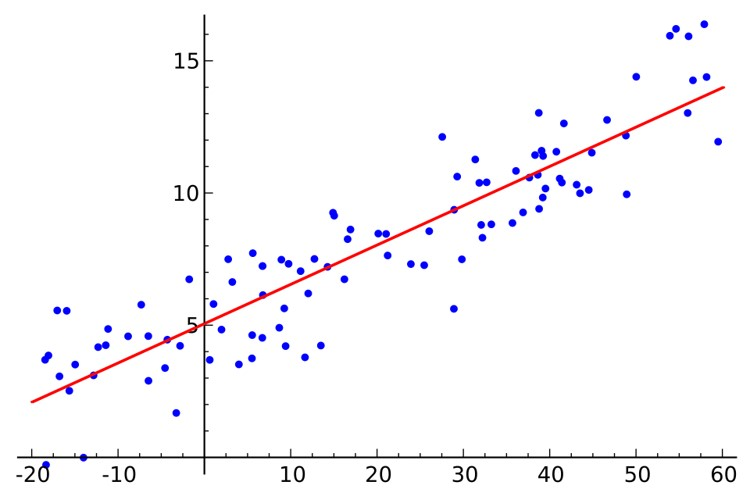
\includegraphics[scale=0.25]{required/Lineare_Regression.jpg}
			\caption{\scriptsize Lineare Basisfunktion [LinWik.2017]}
        	\label{Over and Underfitting}
		\end{figure}
	\end{frame}
	\begin{frame}{KI-Algorithmus}{Implementierungshinweise: Lineare Regression}
		\footnotesize
		\begin{itemize}			
			\item Für eine kompaktere Schreibweise lassen sich $w$ und $t$ in den Parametervektor $\Theta = [w^{\text{T}}, t]^{\text{T}}$ der Dimension $(N+1)$ zusammenfassen und der Eingang $x$ erweitern zu $ \tilde{x} = [x^{\text{T}}, 1]^{\text{T}}$.
			\item Damit gilt: $
				y = \Theta^{\text{T}} \tilde{x} + \eta \text{ mit } \eta \backsim \mathcal{N}(0, \sigma^2) \text{,} $
			\item Die Lösung für den gesuchten Parameter $\theta$ ergibt sich aus dem Minimum der Verlustfunktion. Für die quadratische Verlustfunktion bedeutet dies:
			\begin{equation}
				\theta = \underset{\theta}{\mathrm{argmin}} \left\{\ \frac{1}{M} \sum_{m=1}^M\ (y_m - \theta^{\text{T}} \tilde{x}_m)^2 \right\}\
			\end{equation}
			\item Die Ableitung der quadratischen Funktion hat eine Nullstelle im Minimum					\begin{equation}
				\frac{\delta}{\delta \theta^{\text{T}}} \Bigl( \frac{1}{M} \sum_{m=1}^M\ (y_m - \theta^{\text{T}} \tilde{x}_m)^2 \Bigr) 
				= \sum_{m=1}^M\ -(y_m - \theta^{\text{T}} \tilde{x}_m) \tilde{x}_m^{\text{T}}
				\stackrel{!}{=} 0 
			\end{equation}

		\end{itemize}
	\end{frame}
	\begin{frame}{KI-Algorithmus}{Implementierungshinweise: Lineare Regression}
		Die Lösung ist:
		\begin{equation}
				\theta = \Bigl( \sum_{m=1}^M\ \tilde{x}_m \tilde{x}_m^{\text{T}} \Bigr)^{-1} \Bigl( \sum_{m=1}^M\ \tilde{x}_m y_m \Bigr)
		\end{equation}
		Schreibt man dieses Ergebnis in Matrix-Vektor-Notation, so werden alle Eingänge und Zielwerte aus dem Datensatz $\mathcal{D}$ in der Matrix $\tilde{X}$ und dem Vektor $y$ sortiert. 
		\begin{equation}
			\theta = ( \tilde{X}^{\text{T}} \tilde{X} )^{-1} \tilde{X}^{\text{T}} y
			\hspace{0.5 cm}	
			\text{, mit }			
			\tilde{X} = 
			\begin{bmatrix}
				\tilde{x}_1^{\text{T}} \\
				\tilde{x}_2^{\text{T}} \\	
				\vdots \\
				\tilde{x}_M^{\text{T}} \\		
			\end{bmatrix}
			\text{,  }
			y =	
			\begin{bmatrix}
				\tilde{y}_1 \\
				\tilde{y}_2 \\	
				\vdots \\
				\tilde{y}_M \\
			\end{bmatrix}						
		\end{equation}
	\end{frame}
	
	\begin{frame}{KI-Algorithmus}{Implementierung: Nicht-lineare Basisfunktionen}
		\small		
		\textbf{Motivation}
		\footnotesize
		\begin{itemize}
			\item Die Einschränkung durch Linearität ermöglicht es dem Algorithmus nicht die TTC fehlerfrei darzustellen.
			\item Ein klassischer Fall von Underfitting.
			\item Eine entscheidende Möglichkeit kompliziertere Zusammenhänge darzustellen, ist Nicht-Linearität in die Funktion zu bringen
			\item Eine Möglichkeit sind nicht-lineare Basisfunktionen. 
		\end{itemize}					
		\begin{figure}
			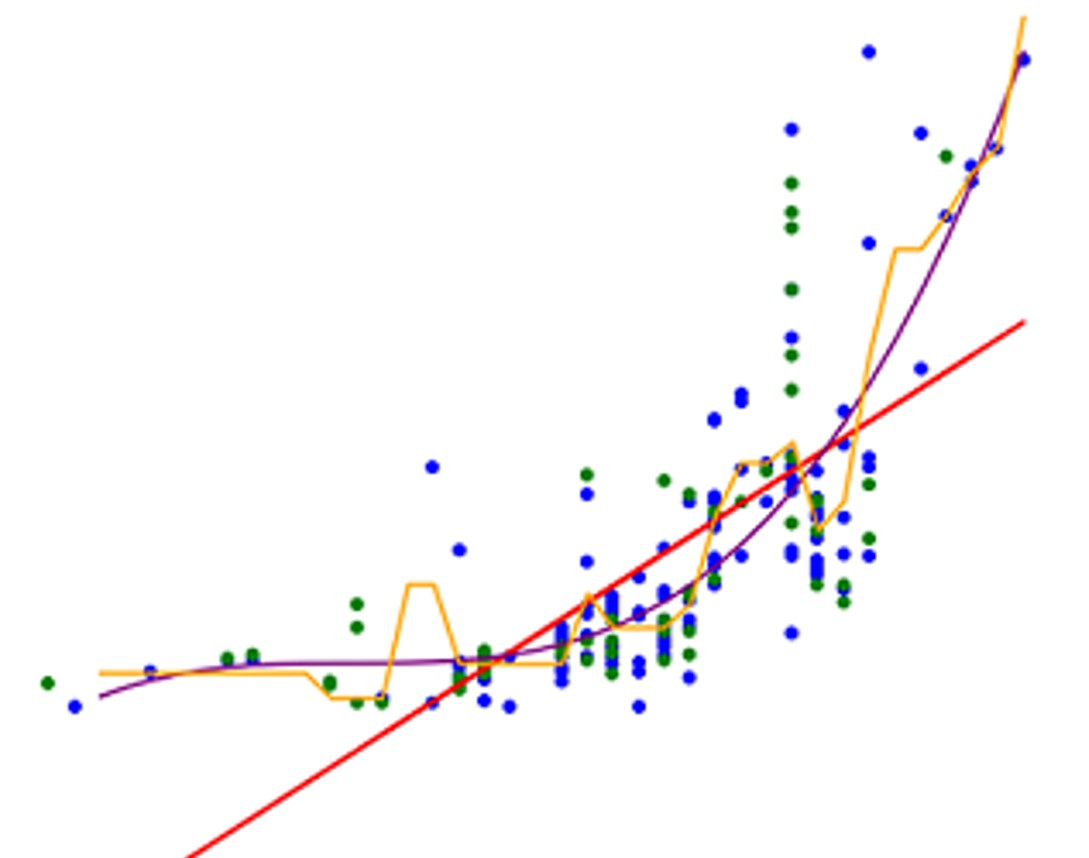
\includegraphics[scale=0.45]{required/Nicht_lineare_Regression.jpg}
			\caption{\scriptsize Verwendung von nicht-linearen Basisfunktionen [NlinWik.2017]}
        	\label{Over and Underfitting}
		\end{figure}
	\end{frame}
	\begin{frame}{KI-Algorithmus}{Implementierung: Nicht-lineare Basisfunktionen}
		\begin{enumerate}
			\item Verwenden Sie die Datensätze der vorhergehenden Aufgabe.
			\item Analog zum beschriebenen Verfahren $x$ soll eine nichtlineare Basisfunktion $\varphi (x)$ verwendet werden. Folgende wird in diesem Fall gegeben:
			\begin{equation*}
				\varphi (x) = 
				\begin{bmatrix}
					\varphi_1(x) & \varphi_2(x) & \varphi_3(x) & \varphi_4(x) & \varphi_5(x) &
					\varphi_6(x) & \varphi_7(x) & \varphi_8(x) & \varphi_9(x)
				\end{bmatrix}
			\end{equation*}
			\item[] mit
			\begin{flalign}
				&\varphi_1 (x) = x_1, \hspace{0.2 cm} \varphi_2 (x) = x_2, \hspace{0.2 cm} 						\varphi_3 (x) = x_1^2, \hspace{0.2 cm} \varphi_4 (x) = x_2^2, \hspace{0.2 cm} 
				\varphi_5 (x) = x_1 x_2, \nonumber \\
				&\varphi_6 (x) = x_1^3,\hspace{0.2 cm} \varphi_7 (x) = x_2^3,\hspace{0.2 cm} \
				\varphi_8 (x) = x_1^2 x_2, \hspace{0.2 cm}  \varphi_9 (x) = x_1 x_2^2 \nonumber
			\end{flalign}
		\end{enumerate}
	\end{frame}
	\begin{frame}{KI-Algorithmus}{Implementierung: Nicht-lineare Basisfunktionen}
		\begin{enumerate}
			\setcounter{enumi}{2}	
			\item Bestimmung von $\theta$ für das neue Regressionsmodell. Test der Ausgabe $\hat{y}$ für den Testdatensatz $\mathcal{D}_{test}$.
			\item Visualisierung des Zusammenhangs von $d$ und $v_x,rel$ zu $\hat{y}$ für das berechnete Regressionsmodell. Visualisierung des Datensatzes $\mathcal{D}_{test}$ im selben Plot.
			\item Integration in die ROS-Pipeline zur Bestimmung der kritischen Zeit TTC in Echtzeit
			\item Zusatzaufgabe: Untersuchen sie die Folgen einer Änderung des Trainingsdatensatzes oder der Basisfunktion
		\end{enumerate}
	\end{frame}
	\begin{frame}{KI-Algorithmus}{Implementierungshinweise: Nicht-lineare Basisfunktionen}
		\begin{itemize}
			\item Basiert auf der linearen Regression, wobei $x$ durch $\phi (x)$ ersetzt wird.
			\begin{equation}
				y = w^{\text{T}} \varphi (x) + t + \eta
				\hspace{0.2 cm}
				\text{mit}
				\hspace{0.2 cm}
				\eta \backsim \mathcal{N}(0, \sigma^2)
				\hspace{0.2 cm}
				\text{und} \hspace{0.2 cm} 			
				\varphi (x) = [ \varphi_1 (x), \varphi_2 (x), \dots, \varphi_H (x)]^{\text{T}} \text{,}
			\end{equation}
			\item[] wobei die Funktionen $\varphi (x)$ nichtlinear sein können
			\item Analog zur vorherigen Herleitung ergibt sich:
			\begin{equation}
				\tilde{\varphi} (x_m)= 
				\begin{bmatrix}
					\varphi (x_m)^{\text{T}} & 1
				\end{bmatrix}^{\text{T}}
			\end{equation}
			\begin{equation}
				\theta = \Bigl( \sum_{m=1}^M\ \tilde{\varphi} (x_m) \tilde{\varphi} (x_m)^{\text{T}} \Bigr)^{-1} \Bigl( \sum_{m=1}^M\ \tilde{\varphi} (x_m) y_m \Bigr) 
			\end{equation}
		\end{itemize}
	\end{frame}
	\begin{frame}{KI-Algorithmus}{Implementierungshinweise: Nicht-lineare Basisfunktionen}
		\begin{itemize}
			\item In Matrixschreibweise ergibt sich:			
		\begin{equation}
			\theta = \Bigl( \tilde{\phi}^{\text{T}} \tilde{\phi} \Bigr) ^{-1} \tilde{\phi}^{\text{T}} y
		\end{equation}
		\item[] mit
		\begin{equation}
			\tilde{\phi} =
			\begin{bmatrix}
				\tilde{\varphi} (x_1)^{\text{T}} \\
				\tilde{\varphi} (x_2)^{\text{T}} \\
				\vdots \\
				\tilde{\varphi} (x_M)^{\text{T}} \\			
			\end{bmatrix}
			\text{,}
			\hspace{0.2 cm}
			y = 
			\begin{bmatrix}
				y_1 \\
				y_2 \\
				\vdots \\
				y_M
			\end{bmatrix}
		\end{equation}
		\end{itemize}	
	\end{frame}			

	\begin{frame}{Quellen}
		Der Aufbau und Inhalt der Folien ist hauptsächlich angelehnt an [Botsch.2020]. Weitere genutzte Quellen sind:
		\begin{itemize}
			\item 1) [Wik.2022] \text{Wikipedia. Lidar. https://de.wikipedia.org/wiki/Lidar. zuletzt abgerufen am 13.05.2022}
			\item 2) [Rummelhard.2017] \text{Lukas Rummelhard, Anshul Paigwar, Amaury Nègre, Christian Laugier. Ground Estimation and Point Cloud Segmentation using SpatioTemporal Conditional Random Field. IEEE Intelligent Vehicles Symposium (IV), Jun 2017, Redondo Beach, United States. pp.1105 - 1110, ff10.1109/IVS.2017.7995861ff. ffhal-01579095}
			\item 3) [GeneSys.2022] \text{ADMA Automotive Dynamic Motion Analyzer with 1000 Hz. 			https://www.leaneautomotive.com/uploads/uMqkUyFj/ProdDescr\_ADMA\_rel\_05.2019.pdf. visited on 13.05.2022} 
			\item 4) [Miller.2022] \text{https://www.wired.com/2014/12/nokia-here-autonomous-car-maps/. Autonomous Cars Will Require a Totally New Kind of Map. visited on 13.05.2022}

		\end{itemize}
\	\end{frame}
	\begin{frame}
		\begin{itemize}
			\item 5) [Breuer.2015] \text{Stefan Breuer, Andrea Rohrbach-Kerl. Fahrzeugdynamik.Mechanik des bewegten Fahrzeugs. 2015. https://doi.org/10.1007/978-3-658-09475-1}
			\item 6) [Hyin.2018] \text{William Hyin. Lidar Obstacle Detection. https://www.codetd.com/en/article/10631576. 2018. zuletzt abgerufen am 13.05.2022}
			\item 7) [Botsch.2020] \text{M. Botsch, W. Utschick. Fahrzeugsicherheit und automatisiertes Fahren. Methoden des Signalverarbeitung und des maschinellen Lernens. 2020. Carl Hanser Verlag GmbH \& Co. KG. eISBN\: 978\-3\-446\-46804\-7}
			\item 8) [Caesar.2020] Caesar et al.. nuScenes: A multimodal dataset for autonomous driving. 2020. arXiv:1903.11027v5	
			\item 9) [Velodyne.2020] Landis Communications Inc.. Velodyne-Lidar-Sensoren ermöglichen 3D-Datenerfassung im neuen NavVis VLX-Kartierungssystem. 2020. zuletzt abgerufen am 13.05.2022
		\end{itemize}
	\end{frame}
\iftrue
	\begin{frame}
		\begin{itemize}
			\item 10) [Bhande.2018] Anup Bhande. What is underfitting and overfitting in machine learning and how to deal with it. https://medium.com/greyatom/what-is-underfitting-and-overfitting-in-machine-learning-and-how-to-deal-with-it-6803a989c76. 2018. zuletzt besucht am 13.05.2022
			\item 11) [Wuttke.2020] Laurenz Wuttke. Machine Learning: Definition, Algorithmen, Methoden und Beispiele. https://datasolut.com/was-ist-machine-learning/. 2020. zuletzt abgerufen am 27.06.2022
			\item 12) [Kozan.2021] Methean Kozan. Supervised and Unsupervised Learning (an Intuitive Approach). https://medium.com/@metehankozan/supervised-and-unsupervised-learning-an-intuitive-approach-cd8f8f64b644. 2021. zuletzt abgerufen am 29.06.2022 
			\item 13 [Aunkofer.2019] Benjamin Aunkofer. Deep Learning. https://data-science-blog.com/blog/2019/01/13/training-eines-neurons-mit-dem-gradientenverfahren/. 2019. zuletzt abgerufen am 29.06.2022 
		\end{itemize}
	\end{frame}
	\begin{frame}
		\begin{itemize}
			\item 14) [ROS.2022] Open Robotics. ROS. https://www.ros.org/. 2022. zuletzt abgerufen am 29.06.2022
			\item 15) [RANSAC.2021] Wikipedia. RANSAC-Algorithmus. https://de.wikipedia.org/wiki/RANSAC-Algorithmus. 2021. zuletzt abgerufen am 29.06.2022
			\item 16) [LinWik.2022] Wikipedia. Lineare Einfachregression. https://de.wikipedia.org/wiki/Lineare\_Einfachregression. 2022. zuletzt abgerufen am 29.06.2022
			\item 17) [NlinWik.2017] Benjamin Aunkofer. Lineare Regression in Python mit Scitkit-Learn. Nicht-lineare Regression mit Scikit-Learn. https://data-science-blog.com/blog/2017/10/17/lineare-regression-in-python-scitkit-learn/. 2017. zuletzt abgerufen am 29.06.2022
		\end{itemize}
	\end{frame}
	\begin{frame}
		\begin{itemize}
			\item 18) [Wang.2019] Bernie Wang. LATTE: Accelerating LiDAR Point Cloud Annotation via Sensor Fusion, One-Click Annotation, and Tracking. 2019. arXiv:1904.09085v1
		\end{itemize}
	\end{frame}

\end{document}

